\documentclass[12pt, oneside, a4paper]{book}

\renewcommand{\baselinestretch}{1.25}
\setlength{\parskip}{5pt}
\setlength{\parindent}{0pt}

\usepackage{hyphenat}
\usepackage[pdftex]{graphicx}
\usepackage{pslatex}
\usepackage{comment}
\usepackage[scaled=1.0]{helvet}
\usepackage[utf8]{inputenc}
\usepackage{blindtext}
%\usepackage{styles/minted}
\usepackage{subfig}
\usepackage[justification=centering]{caption}
\usepackage{url}
\usepackage{titlesec}
\usepackage[T1]{fontenc}
\usepackage{epstopdf}
\usepackage{microtype}
\usepackage{color}



%\usepackage{pgf-blur}

% tick
\newcommand{\tick}{\ding{52}}
\newcommand{\fail}{\ding{55}}

% chapters style
\definecolor{gray75}{gray}{0.75}
\newcommand{\hsp}{\hspace{20pt}}
\titleformat{\chapter}[hang]{\Huge\bfseries}{\thechapter\hsp\textcolor{gray75}{|}\hsp}{0pt}{\Huge\bfseries}
\titlespacing{\chapter}{0pt}{0pt}{1cm}

\begin{document}
\inputencoding{utf8}


\author{Jan Koreň}

\date{}


% *************** Front matter ***************
\frontmatter

%\begin{titlepage}
%
%\setlength{\textwidth}{15cm}
%\addtolength{\hoffset}{-1.7cm}
%\addtolength{\voffset}{-1.8cm}
%
%\vbox to 150mm{
%
%{\fontfamily{phv}\selectfont
%
%\makebox[\textwidth][c]{University of West Bohemia}
%
%\vspace{0.5cm}
%
%\makebox[\textwidth][c]{Faculty of Applied Sciences}
%
%\vspace{0.5cm}
%
%\makebox[\textwidth][c]{Department of Computer Science and Engineering}
%
%\vspace{6cm}
%
%\makebox[\textwidth][c]{\LARGE{\textbf{DIPLOMA THESIS}}}
%
%\vspace{13.3cm}
%
%\makebox[\textwidth][c]{Pilsen, 2013 \hspace{6.5cm} Jan Koreň}
%
%
%
%\vss
%}
%
%
%}
%
%\end{titlepage}

\begin{titlepage}

\font\uni=cmr17 at 22pt
\font\dip = cmb10 at 28pt
\font\nam = cmr17 at 16pt

\addtolength{\voffset}{-1.8cm}

\vbox to 150mm{



\makebox[\textwidth][c]{\uni University of West Bohemia}

\vspace{0.5cm}

\makebox[\textwidth][c]{\uni Faculty of Applied Sciences}

\vspace{0.5cm}

\makebox[\textwidth][c]{\uni Department of Computer Science and Engineering}

\vspace{3.5cm}

\makebox[\textwidth][c]{\dip Master Thesis}

\vspace{2.5cm}

\makebox[\textwidth][c]{\dip Fulltext Search in the Database }
\makebox[\textwidth][c]{\dip and in Texts of Social Networks}

\vspace{12.5cm}

% Problem s hackem
\begin{flushleft}
Pilsen, 2013 \hspace{6.5cm} \theauthor
\end{flushleft}



\vss



}

\end{titlepage}

%\thispagestyle{empty}
\pagestyle{empty}


\chapter*{Declaration}

I hereby declare that this diploma thesis is completely my own work
and that I used only the cited sources. 
%\vspace{20mm}  % vertical space

\theauthor
\thedate

\pagebreak{}


%\thispagestyle{empty}

\chapter*{Acknowledgements}

I would like to thank to my thesis supervisor Ing. Jan Štěbeták for his assistance, support and inspiring suggestions.

%\thispagestyle{empty}
\pagebreak{}


%\thispagestyle{empty}


\chapter*{Abstract}

%\thispagestyle{empty}

This thesis is focused on design and implementation of the full text search in the EEG/ERP Portal. 
This full text search capability includes searching text in the EEG/ERP Portal database as well as in related data from social networks, such as LinkedIn or Facebook. 
With the development of the Portal and the increasing amount of processed data, a proper full text search mechanism for information retrieval is necessary for improving the user experience by enabling efficient do\-cu\-ment retrieval. 

\pagebreak{}

%\vspace{5mm}\\
{\bf Keywords}:
Lucene, Solr, full text search
	
%\thispagestyle{empty}

\vfill\eject

\pagestyle{plain} 

\tableofcontents

% *************** Main matter ***************
\mainmatter

\pagestyle{plain}


\chapter{Introduction}

Accessing required information from a large set of data in a quick and user-friendly manner is no longer an unachievable goal. 
Advancements in the field of information retrieval in the last few decades have made its applications 
very common.
Full text search, as one of such applications, has in fact become an essential part of everyday's life in a modern society.

%, such as full text search, so common 
%that they have become in many cases an essential part of many tasks of everyday's life in a modern society. 
This work deals with the topic of full text search over data belonging to the domain of the EEG/ERP Portal, a piece of software which is being developed at the University of West Bohemia in Pilsen. 

The work is organized into two main parts.
The first part, theoretical part, includes chapters \ref{chap:fulltext}-\ref{chap:eegPortal} and covers theoretical knowledge used throughout the thesis. 
Chapter \ref{chap:fulltext} deals with the problematics of full text search, its core concepts are introduced and a comparison between full text search and relational database systems is made.
Specific open-source full text search engines and libraries are listed in Chapter \ref{chap:engines}.
In Chapter \ref{chap:eegPortal}, the EEG/ERP Portal together with its underlying technologies, which are currently used for its development, are presented. 

The practical part of the thesis is dedicated to creation of the full text search functionality and is formed by chapters \ref{chap:analysis}-\ref{chap:testing}.
% builds upon the theoretical background provided in the theoretical part.
Chapter \ref{chap:analysis} includes analysis of the state of the EEG/ERP Portal before any changes were made, and collecting full text search requirements. 
Based on the requirements, a full text search solution is chosen and the overall system architecture is proposed.
Chapter \ref{chapter:indexDesign} is focused on creating a document model for indexed data, and on all necessary configuration related to indexing and searching these data.
Chapter \ref{chap:implementation} is devoted to implementation of the full text search functionality into the EEG/ERP Portal application.
In Chapter \ref{chap:testing}, unit and integration tests that confirm the functionality of the created code are described.

%Chapter 7 comprises discussion about the chosen implementation and
%potential future work based on results of this thesis.

The final chapter, Chapter \ref{chap:conclusion}, contains a summary of the thesis and presentation of results.



\part{Theoretical Part}

\chapter{Full text Search}

The aim of this chapter is to explain basic concepts applied in full
text search, one of the methods dealing with the problem of searching information.

\section{Information retrieval}

Full text search together with database systems can be considered  as a part of a subdiscipline of computer science known
as information retrieval (IR) \cite{Witten:1999:MGC:323905}.
There is a number of available definitions of information retrieval.
According to \cite{IRDataAlgorithms}, information
retrieval (IR) is loosely defined as

	\begin{quote}
		\textsl{``the subfield of computer science
	that deals with the automated storage and retrieval of documents''}
	\end{quote}

This definition as well as the definitions from other sources (e.g. from \cite{Witten:1999:MGC:323905}) sum up the purpose of IR in a very general way.
While the definition above puts no restrictions to the nature of stored documents in the IR system and therefore comprises both full text search and database systems, there exist stricter IR definitions that do not apply to structured data found typically in relational databases. 
Such definition of IR can be found in \cite{Manning:2008:IIR:1394399}:

	\begin{quote}
		\textsl{``Information retrieval (IR) is finding material (usually documents) of an unstructured nature (usually  text) that satisfies an information need from within large collections (usually stored on computers).''}
	\end{quote}

All IR systems - and full text search engines are no exception - are based on the same architecture which is adapted to requirements the specific systems have. In addition, these systems share common IR terminolgy, whose most important terms are explained in this chapter.

\section{Principles of Full Text Search}

% Ostry text

The field of full text search covers a wide range of topics, including efficient algorithms and data structures in order to enable fast and reliable full text search over large amount (in practice gigabytes) of data. 
It is not the aim of this thesis to provide a deeper, more complex insight into this problematics as the final implementation of the full text search feature will be based on an existing full text search engine. 
However, there are several terms and concepts that must be at least briefly explained so that the reader can fully understand the latter text.


\subsection{Full Text Search Engine Architecture}

As can be seen in schema in Figure ~\ref{fig:fulltext_schema}, full text search engines comprise several steps in order to provide a user with search results to a given \textsl{query}. 
\textsl{Query} is in this case a piece of text to be searched, optionally enriched by special operators which serve for refining the query. It is a \textsl{user} of the IR system who comes up with the query, expecting that the system will fulfill his \textsl{information need} by returning relevant search results.

Search engines need source data to actually perform searching. The basic informational unit which is processed by the search engine and returned to the user in case of match with the query is called \textsl{document}. In this context, a document or a collection of documents inserted to the system are representations of real documents, so a series of data transformations must be made first. These steps are for reasons of clarity not depicted in the schema.
  
\begin{figure}[h]
	\centering
		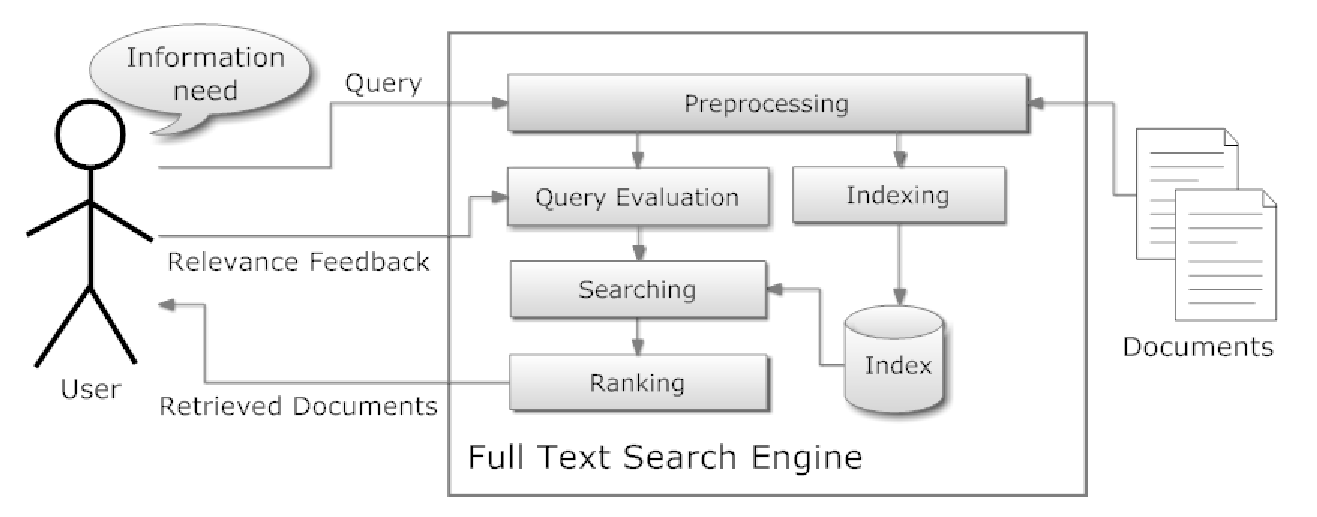
\includegraphics[scale=0.63]{figures/fulltext_schema.eps}
	\caption{IR Architecture Schema. Adapted from \cite{IR:ImplemEvalSearchEng}.}
	\label{fig:fulltext_schema}
\end{figure}

TODO vysvetlit schema, pojmy nize - in progress...

\subsubsection{Preprocessing phase}

Both input query and documents usually undergo several preprocessing steps. These steps, sometimes reffered to as \textsl{filters},   
treat the input text as a stream. 

Tokenization = token stream -> tokens; token normalization -> lowercasing letters, removal of accents, diacritics and so on

separate the text into basic textual units called \textsl{tokens}, in some sources also reffered to as \textsl{words}. These tokens are then operated on. The operations can involve. The result of these operations is a set of terms which are kept in a lexicon of the IR system. 

\subsubsection{Indexing phase}

\subsubsection*{Index}

Index is defined by Frakes \cite{IRDataAlgorithms} the following way: 
	\begin{quote}
	\textsl{``A collection of terms with pointers to places where information about them can be found.''} 	
	\end{quote}
Based on information found in \cite{ManningRaghavanSchuetze08, IRDataAlgorithms, Witten:1999:MGC:323905}, there are three main indexing methods – inverted file, signature file and bitmaps. Based on the comparisons made \cite{Witten:1999:MGC:323905} and in \cite{Zobel:1996:GPC:234889.234891}, using inverted files should be the prefered way due to their faster speed and lower index size required. The remaining two alternatives are recommended to be used only in certain circumstances which are very rare in practice. 

\subsubsection*{Inverted File}

This data structure can be thought of as the well-known index at the end of a book. If we sticked to the IR terminology and characterize it more precisely, we might come up with a more precise characteristics, such as the one found in \cite{Witten:1999:MGC:323905}:

\begin{quote}
		\textsl{``An inverted file contains, for each term in the lexicon, an inverted list that stores a list of pointers to all occurrences of that term in the main text, where each pointer is, in effect, the number of a document in which that term appears.''}
	\end{quote}
	
	To visualize the basic idea of the invered file, Figure  represents a situation of an indexed sentence.
	Obrazek!!!
	
\subsubsection{Query evaluation}

\subsubsection{Searching phase}


\subsubsection*{Boolean query}

\subsubsection*{Ranked query}


\subsubsection{Ranking phase}	


\subsubsection*{Query, Term, Document Operations}

\subsubsection*{Relevance Evaluation}

\subsubsection*{Filters}


% Poznamky

%An IR system matches user queries - formal statements of information
%needs - to documents stored in a database. {[}IRDSA,Frakes{]}
%
%An IR system must support certain basic operations. There must be
%a way to enter documents to a database, change the documents and delete
%them.The must be also some way to search for documents, and present
%them to a user.
%
%and to overcome the informational overload
%
%Though it is possible to keep the index structure in main memory,
%in practice IR databases are usually stored on disk because of their
%size.
%
%Inverted file - a kind of indexed file, the most common solution in
%commercial systems {[}IRDSA,Frakes{]}
%
%The basic item stored in the index 
%
%Todo Lucene in Action and other sources
%
%identify index terms
%
%how to decide if a document matches a query
%
%precision = number of relevant documents retreived divided by the
%total number of documents retreived
%
%recall = number of relevant documents retreived divided by the total
%number of relevant documents
%
%ideally, both parameters should equal to one. This would mean that
%the system returns all relevant documents without introducing any
%irrelevant documents in the results set - impossible to acheive in
%practice.
%
%Improving recall -> precision decreases, likewise improving precision
%at the expense of recall
%
%Furthermore - tradeoff between retreival effectiveness and computing
%cost (key word matching < statistical ranking <\ natural-language
%processing)
%
%Statistical model
%
%Here a document is conceptually represented by a vector of keywords
%extracted from the document, with associated weights representing
%the importance of the keywords in the document and within the whole
%document collection.
%
%Query is modelled as a list of keywords with associated weights representing
%the importance of the keywords in the query.
%

\section{Full text vs. DB search}

Relational database systems and their properties ACID - widely used
for structured data, they are a perfect fit for storing structured
data. As long as these conditions are met relational databases are
a recommended solution for our domain.

traditional search engines - e.g. MySQL databaze. Je zde konstrukce
LIKE (LIKE '\%life\%').

If more terms are searched the underlying query grows in complexity.
Multiple JOIN operations must be used to fetch all data from corresponding
tables, also the query must be written the way to ensure finding the
records with terms not necessarily next to each other as well. As
the query gets more complex, it takes more time to get query results.
Furthermore, the query execution slows down due to the fact that the
query needs to match each term individually.

The query result does not contain any information on the relevancy
of searched terms and found results. Relational database systems simply
output the records matching the criteria.

On the contrary, IR systems provide us with additional relevancy information
of searched terms. Document relevancy is one of the key features of
full text search engines because it is desired to display the results
sorted by their relevance (mostly those most relevant ones are displayed
first).

It is worth mentioning that some DBMS posess native full-text support.
MySQL - keyword FULLTEXT INDEX, for searching on a field, on which full text search will be performed. 
These fulltext indexes are supported only by 
MyISAM engine. They are generally faster than LIKE, however, their usage is limited - vendor lock-in,
moreover, this solution is not unified (implementace,syntaxe se mouhou
can differ, decision to switch to another database could mean interactions to the current system to preserve functionality and scalability. It is bound solely to DBMS - they also lack bigger scaling possibilities and have problems in this area. And it is still slower than external search engines.

{[}IRDSandA,Frakes, p.14{]}:

difference - amount of usable structure in their data objects. Document
generally have less usable structure than the table used by relational
DBMS.

IR - retrieval is probabilistic. No certainity that a retreived document
will meet the informaiton need of the user. (typically, some relevant
documents will be missed, whereas some nonrelevant documents wil be
retreived) vs. DB queries consist of attribute-value pairs that either
match or do not match records in the database.

same - their databases are often very large (can be gigabytes)

same - database volatility - means constant changes as documents are
added, changes or deleted.


\section{Benefits of full text search}

When searching over unstructured data and large data sets, full text
search should be favored to querying relational databases.
\begin{itemize}
\item faster than traditional database search - benefits from word index,
ktery se prochazi pri hledani (jsou pouzity to look up records),
vs. DB - provadi se full table scan
\item found records can be sorted by their relevance. This is called ranking.
\item good performance also over a DB with millions of records
\item ability to skip common words with no additional information. This
depends on the domain languages (in case of English these words include
e.g. the, an, for), search precision can decrease in some cases. 
\end{itemize}
Fulltext pouzijeme, pokud:
\begin{itemize}
\item if there is a lot of unstructured data that are to be looked up
\item it is necessary to get optimized search results.
\item demand for flexible querying
\end{itemize}

\section{Search Engines}

It is a software that is responsible for two steps:
\begin{itemize}
\item building an index on text
\item answering queries by using the created index
\end{itemize}
Compared to databases, it beats them by scalability, relevance ranking,
integration of different data sources (email, web pages, files, database,
...)


\section{Indexing}

Despite various specifics of available search engines, the indexing proces generally consists of several phases.
\cite{Fox:1991:FFA:903195}


\section{Searching Features}

Todo


\chapter{Available Search Engines}
\label{chap:engines}

% http://www.sigir.org/forum/2012D/p095.pdf?searchterm=lucene

% http://stackoverflow.com/questions/737275/comparison-of-full-text-search-engine-lucene-sphinx-postgresql-mysql

% http://php.vrana.cz/fulltextove-vyhledavani-sphinx.php

% http://beerpla.net/2009/09/03/comparison-between-solr-and-sphinx-search-servers-solr-vs-sphinx-fight/

According to the comparisons of fulltext search engines in \cite{MiddletonBaeza} and \cite{SinghSearchEngines}, there are several reasonable options to choose from. 
Unfortunately, there is not enough comparative benchmarks on performance of search engines. Available comparisons are often not so objective since, for example, only the default settings of search engines are used in the tests or just one use case is applied
(as in \cite{SinghSearchEngines}). 
This may lead to false conclusions obtained from these benchmarks because search engines' capabilities might not have been fully demonstrated and tested. 
It is also worth mentioning that some comparisons were made a few years ago and are likely to be out-dated since these technologies evolve quite quickly.
All these experiments showed, however, that database fulltext search possibilities are way too slow \cite{BenchmarkLuceneRelDB,BenchmarkMysqlLuceneSphinx}.

In the following paragraphs the reader can grasp a basic overview on several full text search engines which are considered to be fairly
performant and usable for common full text search scenarios.


\section{Indri}

Indri \cite{IndriHome} is an academic C++ based text search engine
developed at the University of Massachusetts and is a part of the
Lemur Project. The engine is interesting because of its implementation
as it combines inference networks with language modeling. Its API
is accessible also from other languages such as Java or C\#. Great
support of scaling and support of true multithreaded operation, enabling
concurrent adding, querying and deleting documents belong to its main
features. In the technical paper \cite{ComparisonLuceneIndri}
it was shown that Indri is very performant and in comparison with
Lucene it achieves even better results in terms of retrieval effectiveness
for short queries, index size and performance.


\section{Lucene}

Lucene \cite{LuceneHome} is an open source Java-based search library. 
It can enrich applications by its ability to index data and search over them. 
These two main items form what is commonly reffered to as Lucene core. 
Apart from the core, its latest version comprises useful features related to full text search problems (e.g. result highlighting). 
Lucene is highly modularized and its API enables a user to extend its functionality relatively easily \cite{McCandless:2010:LAS:1893016}. 

It stores its index as files on disk. When the search is made, segments of indexes are copied to memory, thus its memory consumption is high and mostly stable.

According to \cite{MiddletonBaeza,ComparisonLuceneIndri}, it belongs to the fastest engines and its performance shines especially
when querying one- or two-word phrases. 
Its small size of index it creates is also a plus when the lack of memory could be an issue.
Thanks to its portability and its active development and active and numerous community, it has become the leading open source search engine used in many successful projects \cite{LuceneWhoUses}.

According to its official documentation \cite{LuceneScoring}, 
\textit{``Lucene scoring uses a combination of the Vector Space Model (VSM) of Information Retrieval and the Boolean model''}.
The Boolean model is used to filter the documents that are then scored.

The current version of Lucene, Lucene 4.0, \textit{,,represents a significant milestone in the development of Lucene due to a number of new features and efficiency improvements as compared to previous versions of Lucene.``} \cite{ApacheLucene4}


\section{Sphinx}

Sphinx \cite{SphinxHome} is an open source search server distributed under GPL license. 
It consists of an indexing tool, which is also referred to as indexer, and a searching daemon. 
Sphinx is written in C++ and is especially designed for indexing database systems (it integrates well with MySQL).
The reason behind its connection with MySQL RDBMS is to enable efficient full-text search on a large amount of database data \cite{aksyonoff2011introduction}.
It allows a user to issue queries with SQL-like syntax for indexing the database content and searching in the index.
Besides database indexing, it also supports an XML format for arbitrary data. 
Considering results from all found benchmarks involving Sphinx \cite{IndriHome,MiddletonBaeza,BenchmarkLuceneSphinxNewer,BenchmarkMysqlLuceneSphinx}, its indexing speed is quick and its search speed belongs to the fastest ones. 
It offers API bindings for several platforms/languages, including Java. 
Among its strengths we can name quick installation and deployment and a perfect online documentation for an open source project. 
Extensibility is quite an issue if our application requires additional features
\cite{esSphinxLuceneSolXapianWhich}. 

\section{Xapian}

According to information found on its official website \cite{XapianHome}, it is an open-source search library written in C++ based on a probabilistic retrieval model. 
It provides a user with bindings that allow to use it from a couple of other languages, including Java, C\# or Ruby. 
Its index size is generally larger when compared to other search engines, but this extra piece of information contained in the index allows Xapian to delete or update a document in a more correct way. 
It is done by storing a list of elements in each document in the termlist table\cite{XapianIndexSize}. 
The benchmarks in \cite{SinghSearchEngines} from 2009 show that its search performance is said to be equally good as the one of Lucene.

\section{Zettair}

Another search engine that received a very positive rating in \cite{MiddletonBaeza} is Zettair \cite{ZettairHome}. 
The comparison in this paper concludes that Zettair has the fastest indexer, provides fast querying speeds and has also the best retrieval effectiveness on average. 
Zettair is being developed at the Australian university and is written entirely in C. 
One of its main features is the ability to handle large data sets (100 GB and more) due to its scalability to large collections \cite{ZettairHome}.

Among its disadvantages belong its inability to index nothing else than text and html and the fact that the index cannot be built in
parallel using multiple machines. 
There are currently no ports to other languages available, so the full text search, when using Zettair, must be implemented in C.


\section{Lucene-based Search Solutions}
\label{sec:luceneBasedSolutions}

Popularity of Lucene is reflected in the existence of several search solutions which are based on this search library.
Because Lucene itself as a search library provides the core functionality, i.e. indexing and searching documents, its direct integration in applications without any additional enhancements can be cumbersome in the most common use cases.
Unless there are special requirements involving access to low-level APIs of Lucene, opting for the already proved search solutions is recommended \cite{Solr3EnterpriseSS}.

The solutions built on top of Lucene can be divided into \textit{search tools} and \textit{search servers}. 
Search tools extend Lucene in a specific way to cover the problem domain and can be embedded to an application in a form of a library. 
They are usually dependent on other technologies which must be included in the target application. 
A widely used example of such search tool is \textit{Hibernate Search}.
Search servers, on the other hand, are fully independent standalone applications which communicate with the application typically by using the HTTP protocol. The representatives of this category are \textit{Solr} and \textit{ElasticSearch}.


\subsubsection{Hibernate Search}

Hibernate Search \cite{HibernateSearchHome} is an enterprise search tool that forms a bridge between Hibernate and Lucene. 
The aim of Hibernate Search is to enable full text search over persistent domain model by overcoming certain mismatches between the domain model and simple Lucene documents.
In order to make Hibernate Search work, Hibernate or JPA must be used as an object-relational mapping between Java objects and database tables. 
% It leverages the power of Lucene for indexing and searching.
% and of Solr (more about Solr can be found in section 3.6.2), whose of useful features and analyzers can be used. 
It manipulates with persisted Hibernate entities and makes them searchable by adding them in the Lucene index. 
By default, Hibernate Search automatically updates Lucene index after an object is saved or updated by using Hibernate.
In order to achieve indexing of Hibernate entities, created model classes must be enriched of specific Hibernate Search annotations for full text search purposes.
Apart from annotating the entities that should be indexed, no extra configuration is needed. 


\subsubsection{Solr}

Solr \cite{SolrHome} is an open source search server built on top of Lucene which runs within a servlet container such as Jetty or Tomcat.
Because it can be considered as a Lucene extension, most of the Lucene terminology is used for Solr as well. 
Unlike Lucene, document fields have to be defined in the application schema file.

Solr extends Lucene by providing many useful features related to full text search, e.g. hit highlighting,
faceted search, rich document handling or the did-you-mean feature, just to name a few. 
Since Solr runs as a separate process, it communicates with applications via HTTP requests, which represent query data, and HTTP responses, representing search results found in the index, by exposing its REST-like API. 
This technology is configuration-driven and in some cases everything can be set up with no need of writing a single line of Java code. 


\subsubsection{ElasticSearch}

Elasticsearch \cite{ElasticSearchHome} is another promising young technology build on Lucene, designed from its early beginnings as a highly scalable solution suitable for big data.

Unlike Solr, it provides a more flexible approach of data definition.
Elasticsearch is a one-man project with a steadily growing community, but compared to Solr, it is relatively immature in terms of some of its features \cite{ElasticSearchComparisonSolr, ElasticSearchComparisonSolrAnother}.

\chapter{EEG/ERP Portal}

This chapter describes the motivation behind the creation of EEG/ERP Portal. Crucial technologies and frameworks that have been used in development of EEG/ERP Portal are also described.

\section{About EEG/ERP Portal}

The EEG/ERP Portal is a web-based application which serves to neuroinformatics researchers as a means of managing, sharing and evaluating measured data. The application also comprises advanced featured designed specifically for the needs of EEG/ERP researchers, such as tools for manipulation with EEG signals.


\begin{figure}
	\centering
		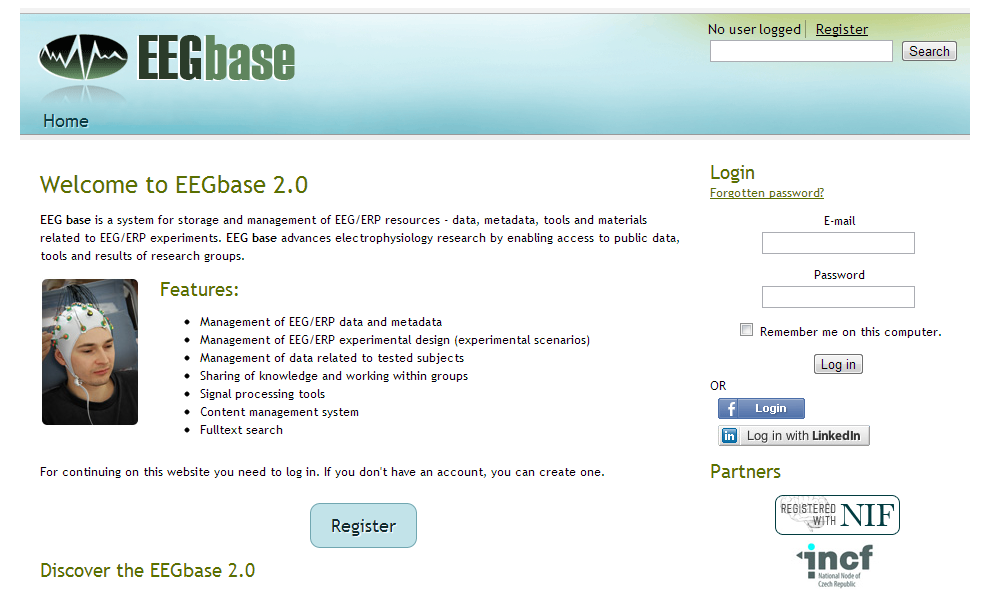
\includegraphics[width=1.00\textwidth]{figures/eegPortal.png}
	\caption{EEG/ERP Portal Welcome Page.}
	\label{fig:eegPortal}
\end{figure}


\subsubsection*{Hibernate}

% Strucne popsat, k cemu je Hibernate a jaky vyuziti ma v portalu. Mozna taky vlozit nejaky schema (z BP?)
Hibernate \cite{Hibernate:Home} is an open-source object-relational mapping framework, whose purpose is to facilitate storage and retrieval of Java domain objects. It is used in EEG/ERP Portal to map its domain model to ...

\subsubsection*{Spring Framework}

% Popsat strucne, jak funguje, jak se vyuziva
The Spring Framework facilitates creating Java-based enterprise applications. It applies a principle called dependency injection which helps to make the classes loosely coupled. The idea of this principle is to let the framework do all necessary wiring of objects, so that the objects can focus on their core responsibilities. 

\subsubsection*{Wicket}

% Popsal v par vetach a uvest, proc se na nej preslo.
... The EEG/ERP Portal's presentation layer is being developed in Wicket by the time of writing this thesis. It is a replacement of JSP pages and Spring MVC. This decision was made due to clearer separation of application logic and markup.





\part{Practical Part}


\chapter{Analysis}
\label{chap:analysis}
% vysvetlit soucasny stav full textu v portalu
% kapitola by mela obsahovat pozadavky
%			co zmenit, co udelat a dodelat, co nedelat 
		% jake jsou pozadavky na vyhledavani, co ma byt vyhledavano
		% jak to ma byt vyhledavano
		% jak to nema byt vyhledavano
		% co by melo vyhledavani umet


This chapter focuses on the analysis of the state of the EEG/ERP Portal before making any changes to its full text search feature.

\section{Current State of Full Text Search}
\label{sec:currentStateFulltext}

%% Jaky je aktualni stav, jeho uvozeni
Currently, the EEG/ERP Portal application uses Hibernate Search as a mechanism to index chosen data stored in Oracle RDBMS.
% Jak je to v soucasne dobe zarizeno. Nedat to radsi do teorie?
Hibernate search provides the annotation interface which serves for indexing purposes. 
A subset of these annotations is used to mark indexed entities and fields withing them which should form the document in the index. Furthermore, a few field annotations enable to configure how the fields are later processed by specifying analyzers to be applied on those fields.

% pridat schema architektury?


By using Hibernate Search to implement full text search, the application is enforced to use Hibernate or JPA for data persistence \cite{Bernard:2008:HSA:1524089}.
Using any other technologies than these two results in a malfunctioning application.
The main drawback of using Hibernate Search in our case the inability to index data from different sources than the database. 
Since one of the requirements is to enable searching data from social networks, the current solution can hardly fulfill this requirement. 


% ???
%We do not have such control over indexed data (?) rozepsat

%% Jake jsou nevyhody soucasneho stavu
% index v pameti - jake jsou vyhody, nevyhody, rizika
In the current state of full text search, the indexed data are stored in memory. 
Keeping an in-memory index provides fast performance of searching because accessing data in memory is much faster than if data are stored on disk. 
A disadvantage of the in-memory index is that these data are lost every time the application server stops.
This is the reason why the index must be created each time the application starts running.
Furthermore, as the size of the index gets bigger, the available amount of memory may be insufficient.
The lack of memory then results in disk swapping which causes serious performance degradation.

Since Hibernate Search uses Lucene as a search library which is responsible for indexing and full text search, the created classes that represent full text search logic in the EEG/ERP Portal make a heavy use of the Lucene API.
Direct Lucene API usage is considered low-level for these purposes, the created code is more difficult to maintain and it is more likely that new bugs are introduced.
In the current state, for example, text highlighting of a subset of found results does not work as expected in some cases.

It is shown in Figure \ref{fig:architBeforeSolr} that the current implementation of full text search is, apart from its dependency on Hibernate, tightly coupled with the whole application. 


\begin{figure}[h]
	\centering
		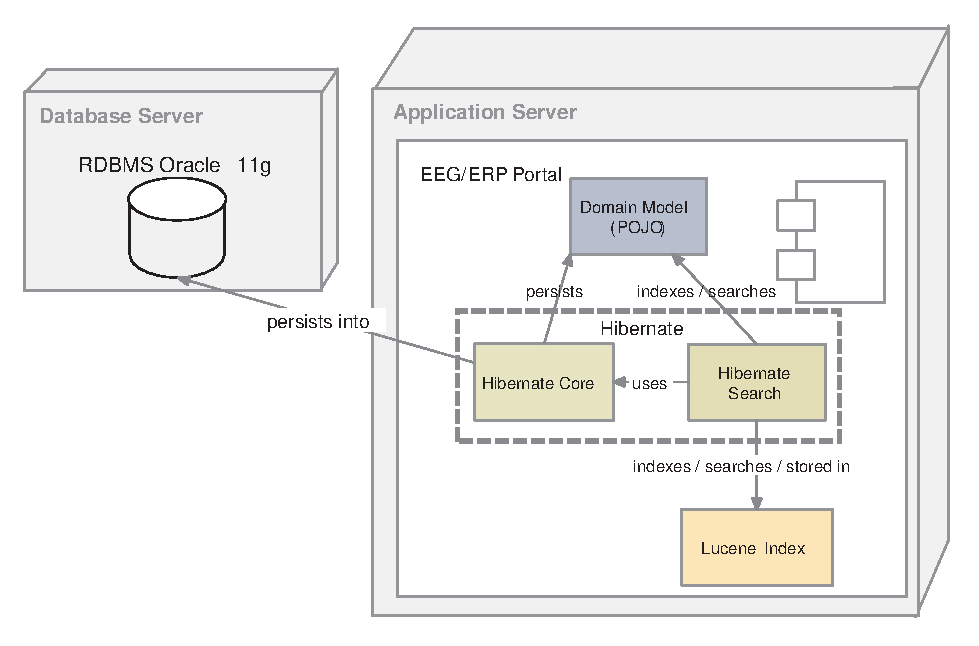
\includegraphics[width=1.00\textwidth]{figures/architBeforeSolr.eps}
	\caption{Architecture with Hibernate Search.}
	\label{fig:architBeforeSolr}
\end{figure}


%With the growing amount of indexed data, the full text search performance might go down as with limited amount of memory there is  not much space for scaling.




\section{Current State of Integration with Social Networks}

Currently, the EEG/ERP Portal is successfully integrated with its LinkedIn group. 
A user can use the EEG/ERP Portal to publish LinkedIn articles as well as to see all of them. 
Users can also log in to the EEG/ERP Portal via LinkedIn. 
Since LinkedIn uses the OAuth 2.0 security protocol for authentication, the OAuth authentication flow is implemented by using Spring Social.

%\section{Search Requirements}

%The current version of the EEG/ERP Portal uses Hibernate Search to implement the fulltext search feature. 
%This framework is sufficient for dealing with input data coming only from a database data source. 
%This is because of the fact that the technology is based on Hibernate, a powerful object-relational mapping framework. Hibernate %Search uses internally Lucene and Solr analyzers to provide the full text search itself.
%The full text search implementation suffers from several issues which are desired to be fixed.
%The highlighting functionality is required to be fixed because it does not work as expected in certain cases. 
%If phrases are searched, found phrases should be highlighted in the text as one piece.

\subsection{Desired Improvements of Full Text Search}


\subsubsection{Appearance}

The user interface of the page with search results should basically remain the same. 
As far as search forms are concerned, it is expected to have:

\begin{itemize}
	\item one search text field on the search page,
	\item another one in the header of each web page so the search can be executed from any page of the website.
\end{itemize}

\subsubsection{Search Functionality}

In terms of search features, there is a need to enable easier navigation among found results.
This is why faceting search based on result categories should be made.
Furthermore, synonym search is desired to allow finding also the results that contain defined synonymic keywords.
Moreover, wildcard search as well as using Boolean AND, OR and NOT operators for querying is required.

\subsection{Social Network Search}
% Duplicitni informace?
Since Hibernate Search is used as a technology responsible, among others, for data indexing, only the data stored in the relational database can be indexed. 
However, articles and other information found in the LinkedIn group of the EEG/ERP Portal have no direct connection to the database, so Hibernate Search cannot reach these data and therefore cannot save them to the index it keeps. 
A possible solution which partially solves this problem would be to keep duplicate records about the articles in the EEG/ERP Portal database. 
Apart from the problem with keeping three copies of basically the same information (the original article published on LinkedIn, its copy in the database and its representation in the Lucene index), those articles published directly from LinkedIn and not from the EEG/ERP Portal via a form would get unnoticed by the application and their corresponding documents in the index would not exist.


\section{Choice of Full Text Search Solution}

From the search engines listed in previous parts of the thesis and technologies on which the EEG/ERP Portal is based, the choice of the search engine can be restricted by the following criteria:

\begin{itemize}
	\item \textit{speed} - Based on the comparison made in chapter \ref{chap:engines}, the most performant search engines are ... and Lucene and all those search solutions built on Lucene. 
	However, speeds of the compared search engines, except for Xapian, differ only slightly. Due to their overall great performance, they can be considered a suitable solution with respect to this criterion.
	\item \textit{integration with the EEG/ERP Portal} - The EEG/ERP Portal is based on Java technologies and this is why search engines providing Java API are easier to be integrated to the working infrastructure and therefore preferred.
	\item \textit{other features and extensions} - Because full text search
engines as they are take care of indexing and searching data, it is desirable to have a set of built-in features, such as result highlighting, faceted search, synonym search or more-like-this search, to make building full text search easier.
 It is taken for granted by the end users to use the full text search with some of such features implemented. 
	\item \textit{independence on data sources} - The chosen search engine must be able to accept data from various sources and to not be limited to only one specific data source, such as relational database. T
	he reason behind this is the mentioned need to index LinkedIn articles as well as to enable further possible indexing scenarios in the future, such as indexing .pdf or XML files.
	\item \textit{independence on other technologies} - This criterion means that the search engine should not rely on a specific technology to be used. 
	Dependence of Hibernate Search on Hibernate or heavy orientation of Sphinx on MySQL may serve as the examples of the search engines which perform well if certain conditions are met, but cannot run or do not perform well if not. 
	\item \textit{community} - Numerous and active developer community also plays a big role in the final choice. 
	The bigger community around the search engine is, the higher is the chance that the engine development will not stop early, new features will be introduced and that found bugs will be resolved quickly. 
	Although relatively new one-man projects can look very promising and their future development is more likely to be managed by a still growing community, their stability is not guaranteed and hence their choice introduces a higher chance that
	A well documented project, many available tutorials and active user groups are a good sign of project stability and ensure that there will be probably someone willing to help to solve given problems.

\end{itemize}

The search engines were evaluated based on these criteria. This evaluations can be seen for reasons of clarity in table \ref{tab:ComparisonOfFullTextSearchEngines}

%TODO MODIFY the table.

\begin{table}[h!]
	\caption{Comparison of Full Text Search Engines.}
	\centering
	\scalebox{0.8} {
		\begin{tabular}{|c|c c c c c|}
		\hline

		\textbf{Search Engine } & \textbf{Speed} & \textbf{Integration} & \textbf{Extension} & \textbf{Independence} & \textbf{Community} \\
		\hline
		Indri & Excellent & \tick & \fail & \tick & 1/5 \\
		\hline
		Sphinx & Excellent & \tick & \fail & \tick & 3/5 \\
		\hline
		Lucene & Excellent & \tick & \tick & \tick & 5/5 \\
		\hline
		Zettair & Excellent & \fail & \fail & \tick & 1/5 \\
		\hline
		Xapian & Good & \tick & \tick & \tick & 1/5 \\ 

		\hline
		\end{tabular}
		}
	\label{tab:ComparisonOfFullTextSearchEngines}
\end{table}

% vysvetleni, co znamenaji jednotliva hodnoceni
It is worth mentioning that the last criterion, Community, cannot be evaluated in an exact manner. This criterion involves the size of mailing lists, the number of search results found on Google, number of related blog posts as well as the number of posts on specialized websites, such as \textit{Stack Overflow}.

The result of the comparison is to base the the EEG/ERP Portal full text search feature on the Lucene search library. As mentioned in Section \ref{sec:luceneBasedSolutions}, the Lucene-based search applications are in practice built by using more sophisticated search solutions (also mentioned in Section \ref{sec:luceneBasedSolutions}). 

\subsection{Chosing Lucene-based Solution}

From the solutions based on Lucene listed in section \ref{sec:luceneBasedSolutions}, it is obvious that Hibernate Search cannot be used due to the reasons that can be found in section \ref{sec:currentStateFulltext}.
Although both Solr and ElasticSearch are likely to be good full-text search solutions for the EEG/ERP Portal, it was decided to choose a more proved and mature alternative (by the time of making this decision, in November 2012). This is why ElasticSearch was favored to Solr.

\section{Using Solr} 

% http://blog.frankel.ch/solr-overview-from-a-beginners-point-of-view

% http://www.optimation.co.nz/optimation-blog/01-03-2011/open-source-faceted-searching-using-solr-and-solrj

% http://www.e-zest.net/blog/about-apache-solr/
	
% \subsection{How Solr Works}


\subsection{Installation}

The whole Solr distribution can be downloaded from the Solr website \cite{SolrHome}. 
It comes in a form of a .war archive. 
Apart from the Solr application itself, it also includes a set of configuration files.



\begin{figure}[h]
	\centering
		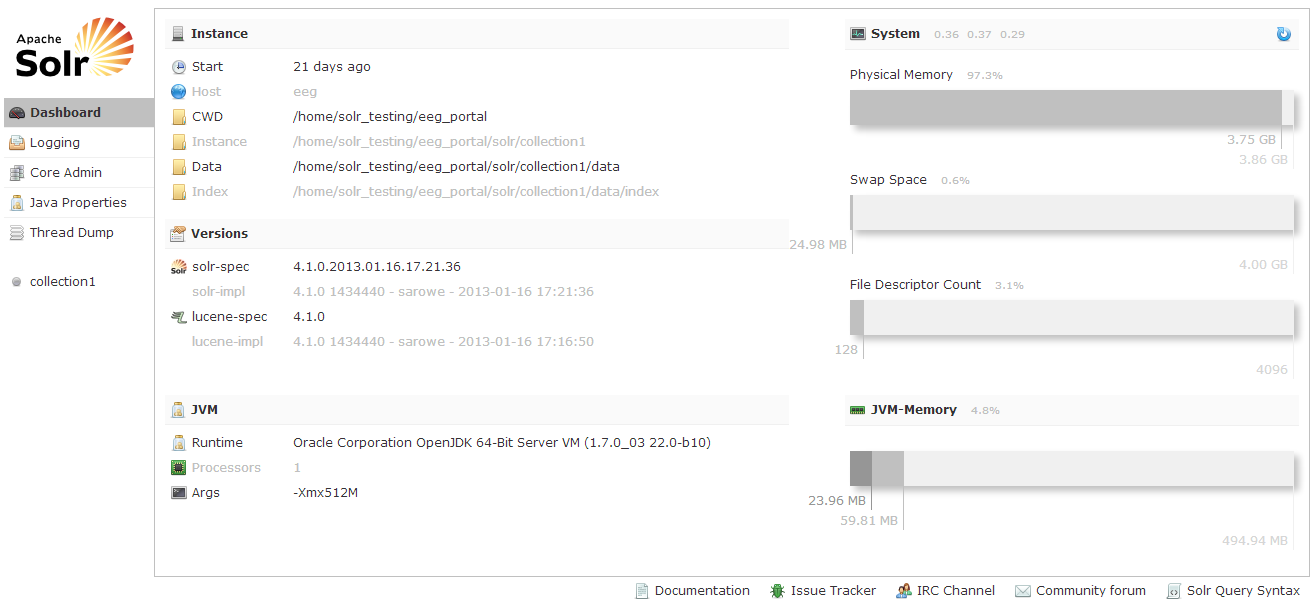
\includegraphics[width=1.00\textwidth]{figures/solrInterface.png}
	\caption{Solr User Interface.}
	\label{fig:solrInterface}
\end{figure}


%\section{Solr and NoSQL}


\subsection{Solr Index}

As told earlier, Solr follows the commonly used search engine terminology. 


\subsection{Solr Configuration}
% co se da nakonfigurovat


% snd HOTOVO
\subsection{General Ways of Integrating Solr}
%jake jsou hlanvi moznosti, uvest je.

There are basically two ways of how to integrate Solr with an existing application. The first way is based on configuration of periodically executed SQL queries that handle database indexing. To do this, the \textit{DataImportHandler} (DIH) tool is used. Another way is to apply a programmatic approach and to use a Java API called \textit{SolrJ}.



\subsubsection{DataImportHandler}
% opet co to je, na co se to pouziva, uvest jeho nevyhody

\textit{DataImportHandler} (DIH) offers fast indexing of data from a variety of sources, including relational databases. 
The extraction of database data for indexing is based on creating custom SQL queries.
The SQL queries serve as a mapping mechanism between query target attributes and document fields.

Although DIH configuration is straightforward to set and its indexing performance is excellent, it has several limitations and disadvantages:

\begin{itemize}

\item \textit{data model changes} - In order to index new data and to enable delta imports, i.e. to index only the changed data since last indexing, it is necessary to add a new time stamp column for each table whose data we wish to index. 
Each record of these new columns contains a time value of the last indexing activity.
Another issue that needs to be solved on the database level is managing deleted database records. There exist several methods to reflect the changes in the index and can be found for example in the Rafał Kuć's article \cite{Solr:DIHDelete}.

%\item \textit{need to manage deleted data} - After deletion of data in the database, certain actions must be taken to enable DIH to reflect these changes in the index. 
%One way to do this is to browse the documents in the index and compare their id values with id values of their matching database records. 
%If a document has no equivalent database record, it means that the record was deleted. 
%After the comparison, redundant documents in the index are identified. 
%This approach does not perform well.
%
%Another way is to add an extra column that captures deletion times. 
%Deletion times together with the record identification are added before the physical deletion of records. 
%DIH can then get all records from the last executed crawl. 
%An appropriate function and before delete trigger must be created for this solution. 

\item \textit{dealing with changes of the database schema} - If the database schema changes, all affected SQL queries must be rewritten in order to index the database correctly again. % SOLR schema changes are related to this point as well. 

\item \textit{code separation} - The logic in the form of the SQL queries is out of reach of the EEG/ERP Portal application logic since the queries must be written in a special configuration file managed by the Solr server.

\item \textit{for indexing only} - DIH is just an indexing tool that creates index documents. It cannot be used for retrieving the documents, so their searching must be implemented in a different way.

\end{itemize}



\subsubsection{SolrJ}
% co to je, co to umi, jake jsou jeho moznosti, proc by se melo pouzit

Solr provides a Java API for integration of Java applications with the Solr server called SolrJ API.
SolrJ client is a recommended way of how to integrate an existing Java application with the Solr server [zdroj]. % najit

SolrJ offers two possible ways of running Solr. Apart from the remote communication with the Solr server provided by the \texttt{HttpSolrServer} class, Solr can also be embedded within the EEG/ERP Portal application by running as the \texttt{EmbeddedSolrServer} instance. 
The latter option is generally not a recommended way to run Solr since Solr is in this case tightly bound to the resources of the running application. % najit info
Following the stated requirements, the embedded version of Solr is not a suitable option for the EEG/ERP Portal either.

\subsubsection{Maven Dependencies}

EEG/ERP Portal uses the Maven build automation tool. 
For both Solr and SolrJ, there are available Maven dependencies that can be added to the Maven \textit{pom.xml} file.
Listing \ref{listing:mavenSolrSolrJ} shows these added dependencies.

\begin{lstlisting}[language=XML, caption={Solr and SolrJ Maven Dependencies.}, label={listing:mavenSolrSolrJ}]
<dependency>
	<groupId>org.apache.solr</groupId>
  <artifactId>solr-core</artifactId>
  <version>4.1.0</version>
  <exclusions>
		<exclusion>
			<artifactId>slf4j-jdk14</artifactId>
      <groupId>org.slf4j</groupId>
    </exclusion>
  </exclusions>
</dependency>

<dependency>
	<groupId>org.apache.solr</groupId>
  <artifactId>solr-solrj</artifactId>
  <version>4.1.0</version>
</dependency>
\end{lstlisting}

% Uvest priklad instanciace solr serveru - beana

% \subsubsection{Running Solr}

% tyka se SolrJ
%HttpSolrServer and EmbeddedSolrServer


\section{Proposed System Architecture}

Based on the text from the preceding paragraphs, a new system architecture was proposed.
The architecture schema is depicted in Figure \ref{fig:solrNewArchitecture}.
Due to the needed interaction with the EEG/ERP Portal, SolrJ API is used as the most flexible alternative.
There are two Solr Server instances running.
One of them is used for maintaining indexed data of the production environment.
The second one is utilized for testing purposes.
Using a separate Solr test server was preferred to its application-embedded version due to the reasons described in previous text.


%% TODO uvest pro co se rozhodnout


\begin{figure}[h]
	\centering
		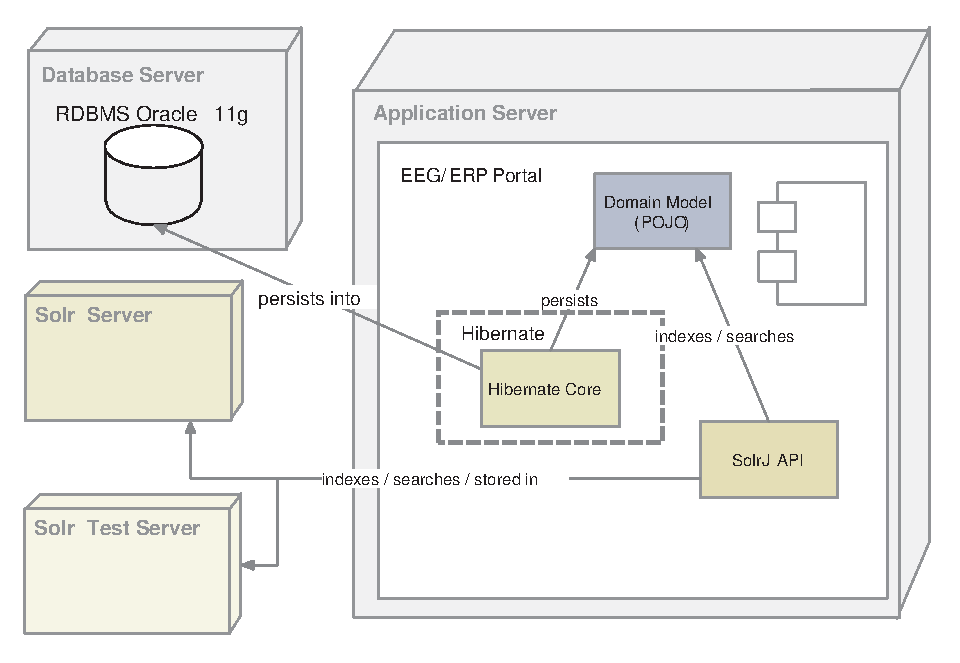
\includegraphics[width=1.00\textwidth]{figures/solrNewArchitecture.eps}
	\caption{Architecture with Solr Included.}
	\label{fig:solrNewArchitecture}
\end{figure}


\chapter{Index Design}
\label{chapter:indexDesign}
% z pozadavku vytvorit strukturu dokumentu uchovavanych v indexu, 
% zminit volbu jednoho indexu misto nekolika indexu

The aim of the following chapter is to design the index structure for the data to be searched. 
Based on the described limitations and collected requirements from Chapter \ref{chap:analysis}, the index structure is proposed and its advantages and disadvantages are mentioned in the text. 


% patri spis do teorie!!!
% <--
%	\section{Index Structure Specifics}
%
% Compared to traditional relational databases, the Solr index lacks the possibility to create more structured content. 
% An analogy to the index would be a single large table in the relational world. 
%As a relational table, index structure is flat and does not allow nesting documents to form hierarchical structures as in the case of document databases like MongoDB.

% ...Index ma plochou strukturu, neumoznuje vnorovat dokumenty
% do sebe, jako v pripade dokumentovych databazi. lze vsak imitovat
% relaci 1:N pomoci multivalued fields, ktere jsou ulozeny ve forme
% pole.
% -->

% http://stackoverflow.com/questions/5584857/solr-documents-with-child-elements

% http://wiki.apache.org/solr/SchemaXml#Dynamic_fields

% http://wiki.apache.org/solr/ExtendedDisMax

% http://people.apache.org/~yonik/presentations/solr4_nosql_apachecon_2012.pdf

% http://stackoverflow.com/questions/5800762/what-is-the-use-of-multivalued-field-type-in-solr

\section{Identifying domain entities}

To design a document structure properly, it is crucial to know what kind of information is going to be searched and what should be displayed to a user.
This is the reason why the EEG/ERP Portal application's domain model must be explored first.

Based on the search requirements, the full text search functionality will be oriented on searching and displaying information about five main domain entities: articles, experiments, persons, research groups and scenarios.


\subsection{Relation to POJO classes}

The corresponding POJO representations of the domain entities are, however, logically split into multiple POJO classes.
Nevertheless, there are several classes which contain the core data belonging to their representing domain entities.
These POJO classes are of our main interest and will be considered parent classes in the full text search context.
There exist one-to-one or one-to-many associations among parent POJO classes and some other, child classes.  
The Solr documents created from the class hierarchy, which is identified in the text below, will mainly consist of textual data.
In practice, it means that mostly \texttt{String} object fields will be stored in the documents.

The following list captures relations between entities of the domain model and their respective parent POJO objects:

\begin{itemize}
	\item \textit{article} - Articles are represented by the \texttt{Article} class. 
	It contains the \texttt{title} and \texttt{text} string fields  that hold values of article title and its text, respectively. 
	Articles can be commented on, so each article may have one or more article comments associated. Text of the comments themselves is contained in the \texttt{ArticleComment} instances. 
	
	\item \textit{experiment} - The \texttt{Experiment} class has the \texttt{environmentNote} field to describe the experiment environment.
	Apart from this field, it also refers to related \texttt{Weather}, \texttt{Disease}, \texttt{DataFile}, \texttt{Hardware} and \texttt{Software} classes that include information about weather, diseases of a tested subject, related data files, and used hardware and software during an experiment, respectively.
	
	\item \textit{person} - The \texttt{Person} class contains a person's name, surname and a note about the person. Although it also has associations to other classes, it is not necessary to include them for indexing and searching purposes.
	
	\item \textit{research group} - The \texttt{ResearchGroup} class keeps a name, title and description of a research group and as in case of the \texttt{Person} class, its structure matches the structure of its domain entity, so no other referenced classes are needed.
	
	\item \textit{scenario} - The class \texttt{Scenario} contains its name, title and description. The class itself corresponds to its domain entity.
\end{itemize}


After inspecting the aforementioned classes, it turns out that there are several fields that most of the objects have in common.
For example, many POJO classes possess the \texttt{title} and \texttt{description} fields.
It is also worth noticing that the class fields \texttt{description}, \texttt{text} and \texttt{note} have a very similar meaning in this context.
This repeatability and similarity of class fields can be conveniently used to create a single type of a Solr document.

On the other hand, there are several class fields that are distinctive only for a few or for a single domain entity (such as the \texttt{temperature} field in the \texttt{Experiment} class or the \texttt{type} field in the \texttt{Hardware} class to specify parameter data type attribute).
% nastesti to nijak moc nevadi, protoze prazdne fieldy v dokumentech nezabiraji zadne misto - doplnit

\subsection{Single vs. Multiple Solr Cores}
% Zduvodnit, proc jsme se rozhodli pro jedno jadro - podobny data

In this case it is necessary to decide whether it is better to create one universal document type and use a single Solr core 
or to use multiple Solr cores for each of the domain classes, each managing its own document type.

Both alternatives have their strengths and weaknesses. 
If separated searching of multiple document types is expected (e.g. in case of different applications using the same Solr server instance or having multiple language mutation of an application) then it is more reasonable to use multiple cores with different schemas, since the core can run independently on each other.
To support searching by using a single search box, the final choice depends strongly on data heterogeneity, i.e. how much different the data in the document types are. According to the Solr wiki \cite{Solr:SchemaDesign}, \textit{``The more heterogeneous (different kinds of data) you have in one field or in one index, the less useful it is.''}

Another factor worth considering is the expected total number of documents. Due to performance gains, it is in practice recommended to split documents to multiple cores if their number stored in a single index exceeds one million [ZDROJ].

In the EEG/ERP Portal, the are some fields of different entities that can be put together under one document field.
Furthermore, the document types tend to be similar % (overall similarity of the document types)
and the total number of documents is not expected to be over one million.
Thus, the choice of having a single core, meaning using a single index, will be preferred.


\section{Ensuring Document Uniqueness}
% je tu problem s unikatnosti id dokumentu, je to potreba resit. jak se to promitne ve schematu

When storing different types of documents under a single index, a problem of document uniqueness arises. 
Although a relational database record can be, for example, uniquely identified by its primary key and a source table, its information about the source table is lost after its corresponding Lucene/Solr document is created.
Hence, the original uniqueness is lost as there might be documents created from records coming from different tables and having the same id. 
This is why a custom mechanism ensuring a unique id for each document was implemented, as can be read in chapter \ref{chap:implementation}.

The need of document uniqueness is reflected on the document level as well.
The following fields related to unique identification of documents were added in the Solr schema file:

\begin{itemize}
	\item \textit{id} - The purpose of the \texttt{id} field is to keep the original object ID value.
	\item \textit{class} - Identifies a type of an indexed document. There are two reasons of having this field. First, in combination with the \texttt{id} field value, it provides a means of identification of a specific object. Therefore, a link to the found record in the application logic can be created. Second, the \texttt{class} field value can be used for displaying a category of a found result to a user as well as for enabling categorization of search results.
	\item \textit{uuid} - This field serves as a unique identifier for each document in the index.
	It consists of two concatenated parts. The first part is the whole class name of an indexed object, the second part is the actual ID value of the object. To provide an example, the \texttt{uuid} value of an article with ID 20 is \texttt{cz.zcu.kiv.eegdatabase.data.pojo.Article20}. 
\end{itemize}

These Solr fields were added to the \texttt{schema.xml} configuration file, whose incriminated lines are displayed in Listing \ref{listing:identificationConf}.

\begin{lstlisting}[language=XML, caption={Configuration of Identification Fields in the Solr Schema.}, label={listing:identificationConf}]
<field name="uuid" type="string" indexed="true" stored="true" required="true" multiValued="false" />         
<field name="id" type="int" indexed="false" stored="true" required="true" multiValued="false" /> 
<field name="class" type="string" indexed="true" stored="true" omitNorms="true"/>
\end{lstlisting}

\section{Proposed Document Structure}

Based on the object hierarchy and fields these objects contain, the following document fields were configured:


\begin{itemize}
	\item \texttt{title} - Title of a parent object.
	
	\item \texttt{text} - A longer textual sequence, such as description or a note, of a parent object.
	
	\item \texttt{name} - It contains a person's name (both first name and last name).
	
	\item \texttt{source} - This field determines a source of indexed documents. It can be set either to \texttt{linkedin}, if a LinkedIn article was indexed, or to \texttt{database}, if a POJO instance was indexed. 
	
	\item \texttt{temperature} - Stores temperature during an experiment.
	
	\item \texttt{param\_datatype} - It represents a data type or another type field of a parent POJO class.
	
	\item \texttt{file\_mimetype} - Stores \texttt{mimetype} values of parent POJOs. In this case, it concerns the \texttt{Scenario} class.
	
	\item \texttt{child\_title} - It is a multivalued field which stores all titles of child objects.
	
	\item \texttt{child\_text} - This field is analogous to the \texttt{text} field. 
	The difference is that it is multivalued and stores all textual values of child objects.
	
	\item \texttt{child\_param\_datatype} - It is used for the same reasons as the \texttt{param\_datatype} field, except that it is used for child object values.
	% dalsi asi nejsou pouzity
	
\end{itemize}

% Because of the length of the part of schema field definitions, all field definitions can be found in Attachment 1.

% UVEST LISTING DO PRILOHY, JESTLI VUBEC

%\begin{lstlisting}[language=XML, caption={Solr Document Structure.}, label={listing:solrDocStructure}]
%<field name="title" type="text_general" indexed="true" stored="true" omitNorms="false"/>
%<field name="temperature" type="int" indexed="true" stored="true" omitNorms="true"/>
%<field name="text" type="text_general" indexed="true" stored="true" omitNorms="false"/>
%<field name="file_mimetype" type="string" indexed="true" stored="true" omitNorms="false"/>
%<field name="param_datatype" type="string" indexed="true" stored="true" omitNorms="false"/>
%<field name="source" type="string" indexed="true" stored="true" omitNorms="false"/>
%<field name="name" type="string" indexed="true" stored="true" omitNorms="false"/>
%<field name="child_temperature" type="int" indexed="true" stored="true" multiValued="true" omitNorms="true"/>
%<field name="child_name" type="string" indexed="true" stored="true" multiValued="true" omitNorms="false"/>
%<field name="child_title" type="string" mindexed="true" stored="true" multiValued="true" omitNorms="false"/>
%<field name="child_text" type="text_general" indexed="true" stored="true" multiValued="true" omitNorms="false"/>
%<field name="child_file_mimetype" type="string" indexed="true" stored="true" multiValued="true" omitNorms="false"/>
%<field name="child_temperature" type="int" indexed="true" stored="true" multiValued="true" omitNorms="true"/>
%<field name="child_param_datatype" type="string" indexed="true" stored="true" multiValued="true" omitNorms="false"/>
%\end{lstlisting}


\section{Result Highlighting}

In order to enable highlighting of search results, the \texttt{solrconfig.xml} configuration file had to be modified.
This modification in a form of default highlighting settings is shown in Listing \ref{listing:highlightConf}.
The fields that will be highlighted are surrounded by the \texttt{str} tag with the \texttt{hl.fl} value of its \texttt{name} attribute (see line 5 in Listing \ref{listing:highlightConf}).

For more information about the used configuration properties, see Chapter \ref{chap:analysis} or refer to the official Solr documentation at [ZDROJ].


\begin{lstlisting}[language=XML, caption={Highlighting configuration.}, label={listing:highlightConf}]
<requestHandler name="/select" class="solr.SearchHandler">
	<lst name="defaults">
		...
		<str name="hl">true</str>
		<str name="hl.fl">title text name source child_title child_text child_param_datatype</str>
		<str name="hl.requireFieldMatch">false</str>
		<str name="hl.usePhraseHighlighter">true</str>
		<str name="hl.highlightMultiTerm">true</str>
		<str name="hl.snippets">10</str>
		<str name="f.text.hl.snippets">5</str>
		<str name="hl.fragSize">100</str>
		<str name="hl.mergeContiguous">true</str>
		<str name="hl.encoder">html</str>
		<str name="hl.simple.pre">&lt;b&gt;</str>
		<str name="hl.simple.post">&lt;/b&gt;</str>
		<str name="f.title.hl.alternateField">title</str>
		<str name="f.text.hl.alternateField">text</str>
		<str name="f.name.hl.alternateField">name</str>
		<str name="f.source.hl.alternateField">source</str>
  </lst>
	...
</requestHandler>
\end{lstlisting}

\section{Autocomplete Support}

In order to enable the autocomplete functionality, an extra document field needed to be added.
The field \texttt{autocomplete} contains all searched phrases which are copied from selected source fields. It is done by utilizing the \texttt{copyField} element for all affected source fields. The excerpt from the schema.xml configuration file can be seen in  Listing \ref{listing:autocompleteConf} below.

\begin{lstlisting}[language=XML, caption={Configuration of Autocomplete.}, label={listing:autocompleteConf}]
<field name="autocomplete" type="text_autocomplete" indexed="true" stored="true" multiValued="true" />
...
<copyField source="title" dest="autocomplete"/>
<copyField source="name" dest="autocomplete"/>
<copyField source="child_title" dest="autocomplete"/>
<copyField source="file_mimetype" dest="autocomplete"/>
<copyField source="param_datatype" dest="autocomplete"/>
<copyField source="source" dest="autocomplete"/>
\end{lstlisting}

\subsection{Autocomplete Field}
% Vytvoreni typu pro autocomplete

A new Solr field designed for text completion was created.
The configuration of the autocomplete field type can be seen in Listing \ref{listing:autocompFieldType}:
The tokens stored in this field are processed both in index and query phase.
Both phases have one tokenizer and one filter class in common.
First, the usage of \texttt{KeywordTokenizerFactory} which, according to the Lucene/Solr documentation, \textit{``Emits the entire input as a single token.''} ensures treating stored field data as a single phrase.
To prevent letter case mismatches, \texttt{LowerCaseFilterFactory} was applied.


During the search phase, the terms related to autocomplete are additionally made by using Solr \texttt{EdgeNGramFilterFactory} class. This class creates n-grams for an input term.
Based on these n-gram terms, the target phrase will be suggested.
The minimal and maximal n-gram lengths are set to 2 and 50, respectively, which allows meaningful phrase suggestions up to the total string length of 50 characters.
In practice, it means that, for example, the filter output for the input string \textit{``hello''} will be 4 tokens: \textit{``he''}, \textit{``hel''}, \textit{``hell''}, and \textit{``hello''}. By typing one of these n-gram tokens, the original \textit{``hello''} string will be suggested.

\begin{lstlisting}[language=XML, caption={Autocomplete Field Type.}, label={listing:autocompFieldType}]
<fieldType name="text_autocomplete" class="solr.TextField" positionIncrementGap="100">
	<analyzer type="index">
		<tokenizer class="solr.KeywordTokenizerFactory"/>
		<filter class="solr.LowerCaseFilterFactory"/>
		<filter class="solr.EdgeNGramFilterFactory" minGramSize="2" maxGramSize="50" />
	</analyzer>
	<analyzer type="query">
		<tokenizer class="solr.KeywordTokenizerFactory" />
		<filter class="solr.LowerCaseFilterFactory"/>
	</analyzer>
</fieldType>
\end{lstlisting}

%It is important to keep in mind that documents stored in the index store information that are to be searched.
%The documents, in fact, capture information, that are not only searched on, but also expected to be displayed.
%It means that it is essential to know the specifics and purpose of full text search in a given domain properly.
%This fact is especially important for document indexation, because documents stored in the index have certatin specifics and limitations that are discussed in following paragraphs.

\subsection{Using Edismax Parser}

The default query parser set in the Solr configuration is \texttt{LuceneQueryParser}. 
Although it offers a lot of possibilities, any Solr syntax mistakes result in \texttt{ParseEx\-ception}. 
To avoid checking every potential state which leads to a syntax error, such as an odd number of parentheses, it is recommended to use \texttt{Extended\-Dismax\-Parser}.
This parser is more tolerant to syntax errors and guarantees that an exception will not be thrown in most of the cases. % almost never thrown
Instead, an empty search result set is returned.
Compared to the default parser, its performance is generally the same [ZDROJ]. % http://solr.pl/en/2010/07/14/solr-and-phrasequery-phrase-bonus-in-query-stage/ 
The Edismax parser is therefore an appropriate choice for common search use cases since it offers the same query possibilities as the default parser. %using Boolean syntax and wildcard search is enabled.
Listing \ref{listing:edismaxConf} depicts the lines responsible for configuration of Edismax parser.

\begin{lstlisting}[language=XML, caption={Configuration of the Edismax parser.}, label={listing:edismaxConf}]
<requestHandler name="/select" class="solr.SearchHandler">
	<lst name="defaults">
		...
		<str name="defType">edismax</str>
		...
	</lst>
<\requestHandler>
\end{lstlisting}



%Reprezentaci dokumentu lze vyresit nekolika zpusoby:
%\begin{itemize}
%\item denormalization of database data
%\item Od Solr 4 podpora join funkce. Dost omezene oproti SQL joinu
%\item nekolik po sobe nasledujicich dotazu, nasledujici dotaz
%bere jako vstup vysledky predchoziho dotazu.
%\end{itemize}
%
%\subsection{Eventual consistency}
%
%za pouziti real-time indexovani. po insertu, updatu, deletu dochazi
%k indexaci prislusneho dokumentu.
%
%Sekvence insert/update/delete a indexace neprobiha atomicky jako transakce.
%Pri chybe muze dojit k nekonzistentnimu stavu (data ulozena,
%indexovana -> OK; data ulozena, ale neindexovana -> nebudou vyhledatelna;
%data neulozena, indexovana -> nalezeny neodpovidajici nebo neexistujici
%vysledky; data neulozena, neindexovana -> DB rollback, puvodni
%zaznam lze vyhledat. 
%Osetreni konzistence v techto pripadech byva netrivialni zalezitost, casto realne resitelna jen castecne. 
%Beznym resenim nekonzistentnich stavu je je ignorovat, protoze nakonec budou po dalsi naplnnovani reindexaci odstraneny. 
%Tim je dosazeno. tzv. eventual consistency.

% vyhodit
% \chapter{Fulltext Search Design}



\chapter{Implementation}
\label{chap:implementation}

This chapter describes the implementation steps to create a full text search. 
It is based on the designed index schema and Solr configuration described in Chapter \ref{chapter:indexDesign}.



% Text nize vyhodit

%Previous parts of the thesis shown that documents in index and records stored in relational database tables serve to different purposes and use cases and hence must be treated differently. 
% The treatment in this context means storing, structuring and saving the data.

%Being aware of the index structure and its specifics, it is almost always necessary to make a kind of transformation from the relational to the index form in order to make the full text search work properly and efficiently. 
%There are several ways to accomplish this goal, one of them involves flattening the relational structure. 
%This leads to denormalized data which is mostly unacceptable in relational databases, but since index is quite different from databases, denormalization is even desired. 
%The main thing one should know when designing an index structure is to know which search results a user expects and how the final representation of full text results should look like.
%
%If an approach of direct 1:1 mapping between entities and documents was chosen, the result would be a corresponding type of document for each entity. 
%The documents are expected to contain only a subset of fields the entities contain.

\section{Solr Spring Integration}
% ukazka, jak se vytvori instance solru pres beanu

To integrate Solr into the EEG/ERP Portal application, SolrJ API is used. 
In order to use the SolrJ API, it is needed to create a \texttt{SolrServer} class instance to enable communication with the remote Solr server. % from the application code.
This is why a Spring bean defining the \texttt{HttpSolrServer} instance was created in Spring application context, as shown in Listing \ref{listing:solrBeanConf}:

\begin{lstlisting}[language=XML, caption={Configuration of the Solr Server Bean.}, label={listing:solrBeanConf}]
<bean name="solrServer" class="org.apache.solr.client.solrj.impl.HttpSolrServer">
	<constructor-arg name="baseURL" value="${solr.serverUrl}"/>
	<property name="connectionTimeout" value="${solr.connectionTimeout}"/>
	<property name="defaultMaxConnectionsPerHost" value="${solr.defaultMaxConnectionsPerHost}"/>
  <property name="maxTotalConnections" value="${solr.maxTotalConnections}"/>
</bean>
\end{lstlisting}

\section{Indexing Data}

It was mentioned in Chapter \ref{chap:analysis} that it was needed to index data coming from different data sources.
Although the ways to build input Solr documents differ, the principle of indexing as the whole is the same for all data sources and can be divided into the following steps:

\begin{enumerate}
	\item A Solr document is created from input data.
	\item A connection between the Solr server and the EEG/ERP Portal application is established.
	\item The document is sent to the Solr server.
	\item Information about the created document is logged.
\end{enumerate}

It is obvious that the steps 2,3 and 4 are common for all kinds of data sources.
To separate common functionality of indexing from the specialized step during which a Solr document is built, the \textit{Template Method} design pattern was used.
By applying this design pattern, the class hierarchy depicted in Figure \ref{fig:indexersUml} was implemented.

\begin{figure}[h]
	\centering
		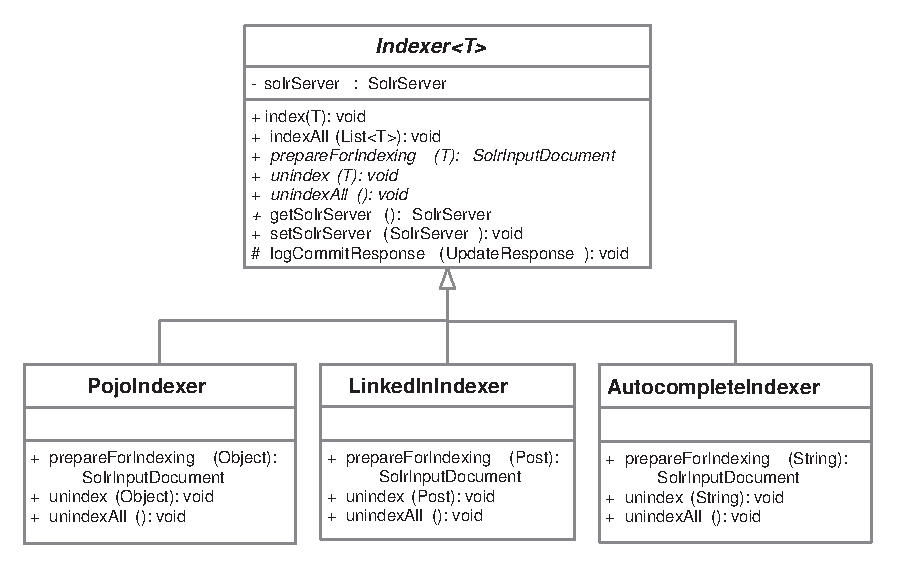
\includegraphics{figures/indexersUml.eps}
	\caption{UML Diagram of Indexer Classes}
	\label{fig:indexersUml}
\end{figure}

The parent abstract class \texttt{Indexer} takes care of performing the generic steps only by providing a \texttt{Http\-Solr\-Server} instance and implementing the \texttt{index()}, \texttt{index\-All()} and \texttt{log\-Commit\-Response()} methods, respectively. 
The step of document creation is handed over to its corresponding implementation of the \texttt{prepareForIndexing()} method  in one of the child classes.
There were three child classes (indexers) created, each being responsible for processing different input data:

\begin{itemize}
	\item \texttt{PojoIndexer} - indexer of POJO classes,
	\item \texttt{LinkedInIndexer} - indexer of LinkedIn articles,
	\item \texttt{AutocompleteIndexer} - indexer of searched phrases that improves the autocomplete functionality.
\end{itemize}

The following sections focus on the provided solutions to creating index documents from input data.
Therefore, three different implementations of the \texttt{prepareForIn\-de\-xing()} method in the classes listed above will be described.


\subsection{Database Indexing}

Generally speaking, the structure of data stored in RDBMS is not suitable for index of full text search engines.
The reasons behind this were already covered in Chapter \ref{chap:fulltext}.
Therefore, a transformation from relational data to document data had to be made.
The domain model and the related POJO classes and their fields of our interest were identified as well, in Chapter \ref{chap:analysis}, so as the expected output in a form of the created Solr schema fields. % which can be found in Chapter \ref{chap:analysis}, too.

\subsubsection{Possibilities of Indexing}
% Jak pomoci SolrJ zajistit v kombinaci s ostatnimi dostupnymi moznostmi integrace s EEG/ERP portalem

The first thing to solve is to choose the way of mapping the POJO fields into Solr schema fields.
By using the SolrJ API, it can be done by the following mechanisms:

\begin{itemize}
\item \textit{ \texttt{@Field} annotation} 
- The purpose of the \texttt{@Field} annotation is to mark the POJO fields that are to be indexed.
In combination with the \texttt{addBean()} and \texttt{addBeans()} methods provided by SolrJ API, Solr documents can be created.

However, this approach can be used only in a limited number of cases where a direct mapping of single-POJO fields is satisfactory.
In more advanced scenarios, such as mapping an object hierarchy to a Solr document, another alternative must be chosen. 
This limitation lies in the inability to use the \texttt{@Field} annotation to mark nested objects or object collections.

Furthermore, the usage of provided annotations brings a problem of ambiguity of mapped objects. 
Documents stored in the Solr index must possess an identifier which is unique across all stored documents. 
Object IDs are unique only in the class scope, so global uniqueness is not ensured. 

% (pouziti Solr UUID nebylo prostreleno). 

\item \textit{using the SolrJ's \texttt{addField()} method} - Although this alternative is not so comfortable as the previous one, it gives more control of creating a Solr document. 
This is because merging multiple POJOs into one Solr document can be achieved.
Nevertheless, using this method only would result in creating a less flexible code which is harder to maintain. 
%for object-document mapping separately cannot provide a universal solution to the given problem.


%\item \textit{aspects} 
%- Aspects are suitable for injecting so-called cross-cutting concerns such as logging and database transactions to avoid spreading the same lines of code across the whole application. 
%In our case, the existing need for indexing domain objects can be realized by simply enriching the base DAO methods responsible for creating, updating and deleting an object. 
%This way the indexing calls happen only in a few known places in code. 
%Introducing an extra aspect for this situation is more likely to be overkill, not to mention added complexity in debugging.

\item \textit{integration with Hibernate Search and using its annotation mechanisms}
 - The core idea of this proposed alternative is to use Hibernate Search capabilities, such as advanced indexing annotation support and automatic indexing of all collected changes, for the initial phase of indexing. 
Though it is possible to combine Hibernate Search and Solr (one of such ways to combine them can be found in \cite{HibSearch:CombinationSolr}), there would be an extra undesired dependency on another technology. 
% The future Hibernate Search version may change its API or some related internal implementation which may result in undesired bugs.
% Furthermore, there is a risk of potential negative side-effects created by this integration due to unsatisfactory analysis
%In addition, to cover indexing of data not present in RDBMS, other indexing mechanisms for these kinds of data would have to be 
% created anyway. 

\item \textit{custom annotation mechanism}
- By exploiting possibilities offered by Java Reflection and combining them with custom Java annotations, a universal solution covering all needs can be implemented.
This way, the problem of creating a Solr document from a class hierarchy, as well as the problem of the same document IDs, can be overcome. 
This alternative is undoubtedly the most challenging one, but its implementation can assure covering all specified needs. 
%gives more freedom than the previously proposed solutions. 

% one cannot be limited by the aforementioned solutions and create a new one that overcomes found problems. 
%It would be desirable to create a solution universal for all domain objects. 
%Inspired by the provided SolrJ annotations. 
% It also involves creating a custom code to implement generating a unique id for each created document.  

% NE! Patri ke zpusobum predavani do indexu
% \item filter - web.xml TODO custom filters

\end{itemize}

% Proc ted budeme mluvit o reflexi
%The last option best fits our needs from all those that are mentioned
For the above-mentioned reasons, it was decided to create a custom annotation mechanism for mapping POJO fields to their respective Solr document fields.
%Therefore, Java Reflection was frequently used to implement the new full text search solution. 
% Java Reflection will be described in the next few lines and its importance in the created code will be clarified.

\subsubsection{Java Reflection}
%Co to je, na co se pouziva, jak se pouziva v implementaci

% http://stackoverflow.com/questions/8392392/adding-to-a-list-via-reflection

% http://www.coderanch.com/t/383648/java/java/java-reflection-element-type-List

Java Reflection was frequently used to implement the new full text search solution. 
This is why its mechanism will be described in a few lines first.
Then, its usage throughout the created code of full text search will be demonstrated.

\subsubsection{Introducing Java Reflection}

Reflection is the ability to inspect the code and make its modifications at runtime. 
It is a feature that makes staticly-typed languages like Java more dynamic. 
Its heavy usage can be found especially in modern frameworks such as Spring or Hibernate, that both use reflection for instantiating classes from information in configuration files. 

A very common use case of reflection in Java is the usage with annotations. 
This combination opens many possibilities of manipulating class metadata. 
In \textit{JUnit 4}, for example, the \texttt{@Test} annotation was introduced. 
The JUnit framework looks up all methods marked by this marker annotation and call them in each execution of running unit tests.

The root class of the Java object hierarchy, the Object class, has the \texttt{getClass()} method providing the corresponding \texttt{Class} object, meaning that all Java classes can be invoked or inspected by means of reflection.

% \subsubsection{Usage of Java Reflection in the EEG/ERP Portal}
% dat priklady, asi i vcetne kodu


%
%The name reflection is used to describe code which is able to inspect other code in the same system (or itself).
%
%One very common use case in Java is the usage with annotations. JUnit 4, for example, will use reflection to look through your classes for methods tagged with the @Test annotation, and will then call them when running the unit test.
%
 %The ability to inspect the code in the system and see object types is Type Introspection. Reflection is then the ability to make modifications at runtime by making use of introspection.
%
 %For example, all objects in Java has the method getClass, which lets you determine its class even if you don't know it at compile time (like if you declared it as Object) - this might seem trivial, but such reflection is not by default possible in less dynamic languages such as C++.
%
%Take for example your typical web.xml file. This will contain a list of servlet elements, which contain nested servlet-class elements. The servlet container will process the web.xml file, and create new a new instance of each servlet class through reflection.
%
%Reflection is important since it lets you write programs that does not have to "know" everything at compile time, making them more dynamic, since they can be tied together at runtime. The code can be written against known interfaces, but the actual classes to be used can be instantiated using reflection from configuration files.
%
%Lots of modern frameworks uses reflection extensively for this very reason. the most comprehensive example is Spring which uses reflection to create its beans, and for its heavy use of proxies
%
%It's useful in a lot of situations. Everywhere you want to be able to dynamically plug in classes into your code. Lot's of object relational mappers use reflection to be able to instantiate objects from databases without knowing in advance what objects they're going to use. Plug-in architectures is another place where reflection is useful. Being able to dynamically load code and determine if there are types there that implement the right interface to use as a plugin is important in those situations.

\subsubsection{Annotation Interface}

In order to inspect classes and collect required field values, the classes as well as the some of the fields within them need to be marked by annotations.
Three different annotations serving different purposes were created:

\begin{itemize}
	\item \texttt{@Indexed} - both class (type) and field annotation that can be used in two ways: When it is used to annotate classes, it marks the parent POJO classes; when used on the field level, it marks child POJO classes or their collections,
	\item \texttt{@SolrField} - a field annotation which marks the fields whose values should be contained in a Solr document,
	\item \texttt{@SolrId} - a field annotation that determines the fields belonging to the unique identifier of indexed classes.
\end{itemize}

Listing \ref{listing:annotationIfaceExample} provides an example of creating the \texttt{@SolrField} field annotation. 
Note that this annotation has the \texttt{name} attribute which serves to specify the matching field name in the Solr schema.
All used Solr field names are defined as enumeration constant values of the \texttt{IndexField} class/enumeration to avoid mistyping them.

\begin{lstlisting}[language=Java, caption={Example of Creating the \texttt{@SolrField} Annotation.}, label={listing:annotationIfaceExample}]
@Target(ElementType.FIELD)
@Retention(RetentionPolicy.RUNTIME)
public @interface SolrField {
    IndexField name();
}
\end{lstlisting}

The usage of the defined annotations is demonstrated on the code of the \texttt{Experiment} class in Listing \ref{listing:annotatedClassExample} (irrelevant lines are omitted). 
It is worth noting that the associated POJO collections, whose fields logically belong to the same Solr document, are annotated accordingly.

\begin{lstlisting}[language=Java, caption={Example of Using Indexing Annotations in the \texttt{Experiment} Class.}, label={listing:annotatedClassExample}]
@Indexed 
public class Experiment implements Serializable {
	@SolrId
	private int experimentId;
	@Indexed
	private Weather weather;
	@SolrField(name = IndexField.TEMPERATURE)
	private int temperature;
	@SolrField(name = IndexField.TEXT)
	private String environmentNote;
	@Indexed
	private Set<Hardware> hardwares = new HashSet<Hardware>(0);
	@Indexed
	private Set<Pharmaceutical> pharmaceuticals = new HashSet<Pharmaceutical>(0);
	@Indexed
	private Set<Disease> diseases = new HashSet<Disease>(0);
	@Indexed
	private Set<Software> softwares = new HashSet<Software>(0);
	...
}
\end{lstlisting}

The first practical application of Java Reflection discussed in this text is strongly related to the created set of annotations.
To leverage the semantics hidden behind the used annotations, it is necessary to use reflection to introduce indexing logic by inspecting these annotated classes.

\subsubsection{Indexing Algorithm}

In the \texttt{prepareForIndexing()} method, it is first found out if the type of a given \texttt{Object} instance, sent as the method parameter, has the \texttt{@Indexed} annotation assigned.
If it does, it can continue traversing the class fields by searching a field with the \texttt{@SolrId} annotation.
The value of such annotated field is used for assembling Solr document fields for later identification of a document.
These document fields were described in Chapter \ref{chapter:indexDesign}.

The next step of the algorithm is of recursive nature and happens on two levels - on the parent and the child level.
In both cases, all values of those fields containing the \texttt{@SolrField} annotation are extracted.
On the parent level, in addition, the fields with the \texttt{@Indexed} annotation are searched to identify the associated child \texttt{Collection} or \texttt{Object} classes which are then traversed.

% The values obtained from the collections are stored in 

The schema in Figure \ref{fig:indexAlgorithm} visually depicts the main idea of the described algorithm.

%TODO
%ma to na starosti metoda prepareForIndexing, ktera si jako parametr bere Object instanci (viz template figure vyse).
%Nejprve se zjisti, zda ma jeho trida prirazenu anotaci @Indexed.
%V kladnem pripade se zjisti, jestli nektery jeji field ma anotaci @SolrId.
%Z hodnoty tohoto fieldu jsou sestaveny document fieldy pro identifikaci dokumentu, ktere byly popsany v kapitola index design.
%Jsou take znazorneny na obrazku indexovaciho algoritmu.
%Pak dochazi k extrakci hodnot vsech fieldu , ktere maji anotaci @SolrField.
%Deje se tak na dvou urovnich - na urovni rodice a na urovni potomku obsazenych v asociovanych objectech nebo kolekcich.
%Nejdrive se prohledava na urovni rodice.
%Krome fieldu s anotaci @SolrField se take prohledavaji ty fieldy s anotaci @Indexed.
%Pro kolekce a objekty takto anotovane


\begin{figure}[h]
	\centering
		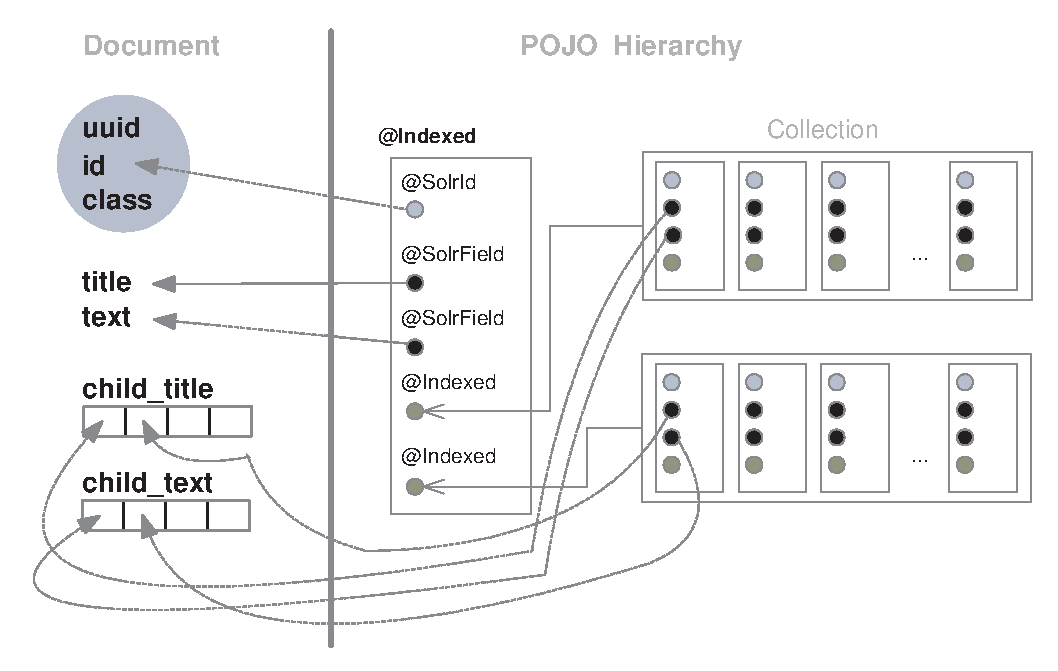
\includegraphics[width=1.00\textwidth]{figures/indexAlgorithm.eps}
	\caption{POJO Indexing Algorithm Schema.}
	\label{fig:indexAlgorithm}
\end{figure}


%All objects annotated by the @Indexed annotation represent the target objects which are required to be searched on.
%Apart from their own object fields, such as title or description of the Scenario object, these objects also contain associated collections of other objects. The fields of objects in the collections need to be indexed as well, since they are related to their respective parent objects. Furthermore, data contained in these nested objects are useful for users to look up required information by using the full text search.

%The conversion of this object structure to the corresponding document in the index is therefore not a straightforward task.
%A transformation from one structure to another must be done.
%If the object structure was flat and there were no associations among the objects, the transformation would be relatively easy to do. In case of independence of all objects, the only thing necessary to do would be to provide a way to determine which fields should be a part of the Solr document, thus to be make searchable.

%Using this approach has some serious disadvantages. 
%It breaks object associations, so it keeps objects separated (isolated).
%Its actual implementation turns out to be quite easy since no additional mapping or traversal needs to be done. 
%Nevertheless, all information which is logically bound to the table record in a form of associations on the database level and in a form of object references on the object level are lost.


\subsubsection{Ensuring eager loading}

In order to make the indexing algorithm work, associated POJO collections, whose object field values are desired to be indexed, have to be already initialized.
This condition, however, is not always met.
As written earlier in Chapter \ref{chap:eegPortal}, it is desired to apply lazy loading of object collections for as many cases as possible. If it is necessary, switching to the eager loading strategy can be done using the following ways:

\begin{itemize}
	\item{change of Hibernate mapping configuration}
	- This modification involves setting the \texttt{lazy=''false''} attribute for collections to be eagerly loaded. 
	It means that all affected 1:N relationships are always loaded together with the parent object. 
	This approach is not very flexible, because no proxies are created and the lazy loading behavior cannot be therefore configured at runtime.

	\item {custom HQL queries or Hibernate criteria that force eager fetching}
	- If HQL queries are used, one can specify eager fetching using the \texttt{fetch} keyword. 
	In case of using the Criteria Query API, the \texttt{setFetchMode()} method with its fetch mode attribute set to \texttt{FetchMode.EAGER} does the job.
	This alternative is more flexible than the previous one since lazy object initialization, which is set by default, is overridden by the eager fetch mode. 
	The created proxy objects call the associated real objects to fetch necessary data. 
	The drawback of this solution is the necessity to create custom HQL queries or Hibernate criteria for each entity that will cause collections to be lazy-loaded. As the created queries can differ a lot, it is very difficult to apply this solution in a generic way.
	

	\item {usage of the \texttt{Hibernate.initialize()} method} 
		- This method is used to initialize lazy-loaded collections. Its parameter takes an object that is to be fetched to the parent object.
		The method also ensures that all already initialized objects will be omitted.
		The power of the \texttt{Hibernate.initialize()} method lies in its universality. When used together with Java Reflection, a universal solution enforcing eager loading of collections for any POJO object can be achieved. 
		It can be used even after the session is closed.

\end{itemize}


Based on the aforementioned possibilities and current requirements, using the \texttt{Hibernate.initialize()} method in combination with the power of Java Reflection was preferred. 

This decision leads to modification of the \texttt{SimpleGenericDao} class. It was enriched of a new generic method which implements the chosen eager loading strategy. 
The method, namely the \texttt{getAllRecordsFull()} method, works on the principle of finding out all proxied object fields, i.e. those fields which are not initialized yet.
All fields are accessed by reflective calls of their respective getter methods available in a given class.
The fields are then initialized by adding them as the parameters of subsequent \texttt{Hibernate.initialize()} method calls.

The following Listing \ref{listing:eagerByReflection} shows the implementation of eager loading on demand described in the paragraph above.

% Dat kod te metody do prilohy?
\begin{lstlisting}[language=Java, caption={Enforcing Eager Loading by Using Java Reflection.}, label={listing:eagerByReflection}]
public List<T> getAllRecordsFull() {
	List<T> records = getAllRecords();
	for(T record : records) {
		Method[] methods = record.getClass().getDeclaredMethods();
    for (Method method : methods) {
			if(method.getName().startsWith("get") && !method.getReturnType().isPrimitive()) {
				try {
					initializeProperty(method.invoke(record));
        } catch (IllegalAccessException e) {
					log.error(e);
        } catch (InvocationTargetException e) {
					log.error(e);
        } catch (Exception e) {
					log.error(e);
        }
      }
    }
  }
  return records;
}

...

protected void initializeProperty(Object property) {
	if(!Hibernate.isInitialized(property)) {
		getHibernateTemplate().initialize(property);
  }               
}
\end{lstlisting}



\subsection{LinkedIn Indexing}

% The following text uses 

% dat spis do teorie !!!
%\subsubsection{REST}
%
%leverages existing technologies - HTTP GET update - POST or PUT. It has taken the advantage of the HTTP protocol itself to describe the action that should be performed on a given resource.

\subsubsection{Using Spring Social}
% Proc primy vyuziti nestaci, jak vyresit, priklad, co se implementovalo

The methods provided by Spring Social are set to give a user a set of default fields that are appropriate for some use cases. 
Although it is very convenient to have such layer of abstraction, sometimes there is a need to obtain other fields or to omit some of them. 
For example, if the Spring Social method for getting all articles in a group is called, some information, such as article summaries and their time stamps, are missing. 
In such cases, a custom LinkedIn REST call must be created and put as a parameter of the \texttt{restOperations().getForObject()} method provided by Spring Social.
The call can contain field selectors which are used to specify which fields to return in the response.
The following example in Listing \ref{listing:linkedinRest} shows the usage of field selectors in the REST call.
The REST call in the listing gets full information about twenty latest LinkedIn articles published in the EEG/ERP Portal group.
Note the \texttt{{group-id}} placeholder which is later substituted by the real value of the EEG/ERP Portal group ID.

%Group.GroupPosts groupPosts = linkedin.restOperations().getForObject(
	%"http://api.linkedin.com/v1/groups/{group-id}/posts" +
  %":(creation-timestamp,title,summary,id," +
  %"creator:(first-name,last-name))?" +
  %"count=" + count +
  %"&start=" + start +
  %"&order=recency",
  %Group.GroupPosts.class, groupId);
%return groupPosts.getPosts();

\begin{lstlisting}[language=HTML, caption={Example of a LinkedIn REST API call.}, label={listing:linkedinRest}]
http://api.linkedin.com/v1/groups/{group-id}/posts:
(creation-timestamp,title,summary,id,creator:(first-name,last-name))?
count=20&start=0&order=recency"

\end{lstlisting}

In the application code, LinkedIn REST calls are wrapped in the methods of the \texttt{LinkedInManager} class. The class includes these methods using direct LinkedIn REST calls:

\begin{itemize}
	\item \texttt{getGroupPostsWithMoreInfo(int count, int start)} - It uses a very similar REST call as the one in Listing \ref{listing:linkedinRest} to obtain LinkedIn articles. 
	The number of retrieved articles and the index position of the first retrieved articles are defined in the method parameters. 
	% \item \texttt{getLastPost()} - This method returns the last post added to the EEG Portal LinkedIn group.
	% \item \texttt{getLastPostId()} - Returns the id value of the last post added to the EEG Portal LinkedIn group.
	\item \texttt{getPostById(String id)} - Gets a LinkedIn post by its unique ID.
	\item \texttt{deletePost(String id)} - Deletes a post by specifying its ID as the method parameter.
\end{itemize}

Apart from the methods mentioned above, the following methods were added to the \texttt{LinkedInManager} class as well:
% jsou pouzity ve spojeni s indexovanim

\begin{itemize}
	\item \texttt{getLastPost()} - This method returns the last post added to the EEG Portal LinkedIn group.
	\item \texttt{getLastPostId()} - Returns the id value of the last post added to the EEG Portal LinkedIn group.
\end{itemize}

Usage of these methods is related to indexing LinkedIn articles which are created by using the EEG/ERP Portal.

\subsubsection{Article-document Mapping}

Compared to POJO-document mapping, mapping from the LinkedIn article to the created Solr document structure is straightforward.
Received LinkedIn Post objects store only unique string ID, article title and summary values, so converting them to Solr documents involves copying these values to the respective \texttt{uuid}, \texttt{text} and \texttt{title} document fields.
Apart from that, the document fields \texttt{class} and \texttt{source} must be populated in order to find these articles successfully while doing a full text search.


\subsection{Indexing Searched Phrases}
% proc vubec a jak implementovano

It was decided to make searched phrases indexable.
Indexing them enables the phrases to appear in the autocomplete box.
Moreover, by indexing search phrases, search frequency of each phrase can be found out and stored together with the phrase in the document.
This way, indexed phrase frequencies enable suggesting the most queried phrases first.

Internally, a phrase and its search frequency are stored together in the \texttt{autocomplete} Solr field and are separated by the number sign (\#) symbol.

\subsection{Changing Indexed Data}

When some data stored in RDBMS are removed or edited, the made changes need to be reflected in the Solr index.
In case if parent POJO objects are changed, the analogous document changes can be performed by using the indexer's \texttt{index()} and \texttt{unindex()} methods. The first method simply overwrites a stored document having the same \texttt{uuid} field as the new inserted one. The latter method removes a document determined by an object set as the method parameter.

However, child objects have no direct document equivalents, because they form only a part of the documents of parent objects.
Although partial updates are possible since Solr 4.0, they are not implemented.
The reasons of not implementing them are the following:
	
	\begin{itemize}
		\item It is expected that the EEG/ERP Portal application is designed to treat the child objects always in the context of their parent object.
		\item Adding the partial update support brings a new level of complexity into the application. Due to the application nature and its requirements, the added complexity was not worth the effort in this case.
	\end{itemize}

Nevertheless, if a change of a child object happens, the index will become inconsistent.	
This is why periodic indexing of database data has to be ensured to prevent potential inconsistent index states and to reach the so-called \textit{eventual consistency}.

Almost the same applies to LinkedIn articles where the problem is extended by adding, updating and removing the articles by the means of the LinkedIn website. 

\subsection{Periodic indexing}

\subsubsection{LinkedIn Articles}
There are two ways to add an article to the EEG/ERP Portal group: either indirectly by filling in the form on the EEG/ERP Portal website or directly from LinkedIn.

In the first case, articles can be indexed immediately after publishing them because their times of publishing are known due to the interaction with the EEG/ERP Portal. 
The last published article in the LinkedIn group can be fetched by the means of LinkedIn REST API and then modified by the indexer so that information about the article can be added to the index.

The latter case is more complicated as there is no interaction with the EEG/ERP Portal. 
So in order to index all LinkedIn articles, the article data must be retrieved first.
It can be done by using LinkedIn REST API calls to receive their object representation.
Since there is no available information of when articles are uploaded to LinkedIn, the REST calls must be done periodically.
This way, periodic indexing of all articles published on LinkedIn can be achieved.

Although the obvious disadvantage of periodic indexing is the existence of a delay between publishing times of some articles and their indexing times (which is equal to the indexing period in the worst case), this method assures that all articles get indexed in the end.

\subsubsection{Scheduling in Spring}

% http://javahunter.wordpress.com/2011/05/05/cronscheduler-in-spring/

The Spring Framework has a native support of task scheduling and asynchronous calls. 
Since its version 3.0, methods can be scheduled and also run asynchronously by using annotations, namely the \texttt{@Scheduled} and \texttt{@Async} annotations. 
The first mentioned annotation, when added to a method, makes the method schedulable by Spring. 
Usage of this annotation is restricted to the void methods with no parameters. 
The \texttt{@Scheduled} annotation has to contain a piece of metadata to tell Spring how to plan the method scheduling. 
Currently there are three available attributes for the \texttt{@Scheduled} annotation, from which the most flexible option is specifying a cron expression to trigger a task as shown on the following lines:

\begin{lstlisting}[language=Java, caption={Example of a Cron Expression.}, label={listing:cronExpression}]]
@Scheduled(cron=* 0 22 * * SAT-SUN)
public void indexAll()
\end{lstlisting}


This way, the method \texttt{indexAll()} will be scheduled to run always at 10 pm only on Saturdays and Sundays. 
The cron syntax allows a user to create more sophisticated scheduling scenarios, but discussing the syntax is out of scope of this work. 
Since Spring is internally using Quartz as a scheduler, an interested reader can find all necessary information about the syntax in the Quartz documentation \cite{QuartzDoc}.

The \texttt{@Async} annotation is used to mark the methods to be invoked asynchronously.
It is very easy to use for methods having void return values.
Listing \ref{listing:asyncAnnotation} shows the usage of the \texttt{@Async} annotation for the \texttt{indexLinkedIn()} and \texttt{indexDatabase()} methods that handle LinkedIn-articles and RDBMS indexing, respectively.


\begin{lstlisting}[language=Java, caption={Using the \texttt{@Async} Annotation.}, label={listing:asyncAnnotation}]
@Async
public void indexLinkedIn()
...
@Async
public void indexDatabase()
\end{lstlisting}

In order to enable annotation-based scheduling, it is necessary to add a new element in the application context file as well as the \texttt{task} namespace to which the element belongs (see Listing \ref{listing:springTaskNs}).

\begin{lstlisting}[language=XML, caption={Using task namespace}, label={listing:springTaskNs}]
<xmlns:task="... http://www.springframework.org/schema/task" 
xsi:schemaLocation="... http://www.springframework.org/schema/task/spring-task.xsd">
...
<task:annotation-driven executor="indexingExecutor" scheduler="indexingScheduler"/>
\end{lstlisting}

The annotation-driven element requires \texttt{executor} and \texttt{scheduler} attributes to be set to handle tasks represented by methods marked by \texttt{@Async} and \texttt{@Scheduled} annotations, respectively.
The related lines can be seen in Listing \ref{listing:settingSpringExecSched}:

\begin{lstlisting}[language=XML, caption={Setting Spring Executer and Scheduler.}, label={listing:settingSpringExecSched}]
<task:executor id="indexingExecutor" pool-size="5"/> 
<task:scheduler id="indexingScheduler" pool-size="1"/>
\end{lstlisting}


%
%,,Notice that an executor reference is provided for handling those
%tasks that correspond to methods with the @Async annotation, and the
%scheduler reference is provided for managing those methods annotated
%with @Scheduled.``

	
\subsection{UML Class Diagram}

The relationships among classes that create the indexing part of the full-text search are depicted in Figure \ref{fig:umlDiagramIndexing}.

\begin{figure}[h]
	\centering
		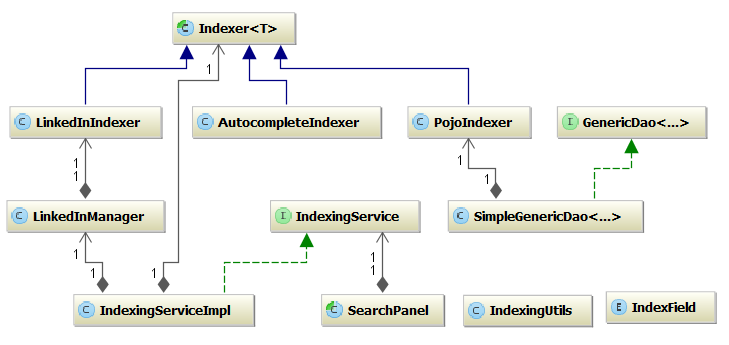
\includegraphics[width=1.00\textwidth]{figures/diagram_indexing.png}
	\caption{UML Class Diagram of the Indexing Part.}
	\label{fig:umlDiagramIndexing}
\end{figure}

There can be seen these most important classes:

\begin{itemize}
	\item \texttt{IndexingService} - Contains the indexing methods \texttt{indexDatabase()} and \texttt{indexLinkedIn()} described above that handle periodic indexing.
	\item \texttt{Indexer} - Direct usage of its \texttt{index()} and \texttt{unindex()} methods is made when any of POJO objects or LinkedIn \texttt{Post}s is created, updated or deleted. Thus every domain object must be associated with its indexing in the first two cases and its removal from the index in the last case. It is achieved by calling these methods in the \texttt{create()}, \texttt{update()} and \texttt{delete()} in the \texttt{Simple\-Gene\-ric\-Dao} class and in the \texttt{publish} and \texttt{deletePost} methods of the \texttt{Linked\-In\-Ma\-na\-ger} class.
\end{itemize}

	
\section{Searching}

This section deals with the search user interface.
The interface was implemented by using the Wicket Framework.

% byly vytvoreny komponenty, ktere byly do sebe vnorovany
% hlavni logika vyhledavani je obsazena ve tride FulltextSearchService

\subsection{Search Logic}

Most of the search logic can be found in the \texttt{FulltextSearchService} class.
This method is responsible for: 

\begin{itemize}

	\item returning search results for a given query - method \texttt{getResults\-ForQuery()}
	\item returning suggested search phrases for autocomplete - method \texttt{getText\-To\-Auto\-complete()}
	\item returning a total number of found documents for a given query - method \texttt{getTotal\-NumberOf\-Documents\-ForQuery()}
	\item faceting by document categories - method \texttt{get\-Category\-Fa\-cets(String solrQuery)}

\end{itemize}

The method \texttt{getResultsForQuery} returns \texttt{FullTextResult} objects that represent results received from the Solr server for a query.
The \texttt{FullTextResult} class, in fact, contains fields that match those contained in the Solr document, i.e. the fields whose information has a value for users - document title, text fragments with highlighted searched keywords, type of the document, class of a Wicket target page which contains further details, id of a corresponding POJO, and time of indexation.

\subsection{Full-text Search User Interface}

Objects of the \texttt{FullTextResult} class are handed over to classes that form the full-text search user interface.  

Namely, these classes include:

\begin{itemize}
	
	\item \texttt{SearchFacets} - It creates faceted search by showing number of found results for each of the document categories, allowing to filter the found results by the document category. Uses the \texttt{FacetCategory} class - name, count, and enumeration \texttt{ResultCategory}. % TODO
	
	\item \texttt{SearchPanel} - This abstract class represents a search panel that provides all necessary functionality, including the autocomplete capability. 
The reason why the class is abstract is that Wicket enforces to have a separate class for each HTML markup. 
Since it is required to have one search panel in the page header and another one, which is different by appearance, in the search page, their corresponding classes had to be created.
There is the \texttt{MenuSearchPanel} class for the search panel located in the page header. For displaying the search panel in the search page, the \texttt{PageSearchPanel} class was made.
	
	\item \texttt{SearchResultPanel} - It is responsible for displaying search results. % which are populated to the Wicket \texttt{DataView} component. 
	The search results are rendered by using the created \texttt{Search\-Result\-Data\-Provider} class that communicates with the \texttt{Fulltext\-Search\-Ser\-vice} class to obtain the matching \texttt{FullTextResult} instances. Besides that, it also displays the number of found results per each document category by utilizing an instance of \texttt{SearchFacets}.
	
	\item \texttt{SearchPage} - It represents the search page. It uses the listed \texttt{Search\-Re\-sult\-Pa\-nel} and \texttt{Page\-Search\-Panel} classes to display necessary information. 
	
\end{itemize}


% \subsection{Handling synonyms}
%  jak konfigurovat, moznosti, ukazka --> DAT DO INDEX DESIGN
%  nevyhody defaultniho reseni v Solru, jak je mozno vylepsit --> DAT DO INDEX DESIGN

% http://stackoverflow.com/questions/4493140/how-to-reload-synonyms-txt-in-solr

% http://nolanlawson.com/2012/10/31/better-synonym-handling-in-solr/

% http://www.quora.com/Apache-Solr/How-can-I-load-the-synonyms-words-from-MySQL-in-Solr


%\subsection{Search Results}

\subsection{UML Class Diagram}

The described classes related to searching documents and associations among them are depicted in the UML class diagram in Figure \ref{fig:umlDiagramSearching}

\begin{figure}[h]
	\centering
		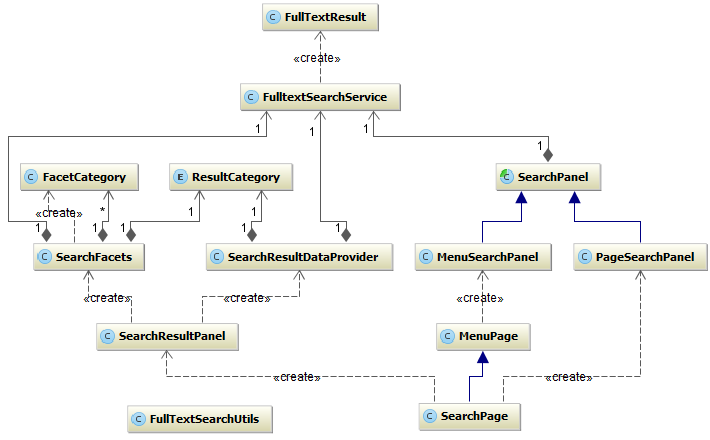
\includegraphics[width=1.00\textwidth]{figures/diagram_search.png}
	\caption{UML Class Diagram of the Search Part.}
	\label{fig:umlDiagramSearching}
\end{figure}

%\subsection{Search Form}

%\subsubsection{Autocomplete}

%\subsubsection{Highlighting}

%\subsubsection{Faceting}

% http://searchhub.org/2009/09/02/faceted-search-with-solr/

% http://lucene.472066.n3.nabble.com/Highlighting-in-SolrJ-td495857.html

% http://www.optimation.co.nz/optimation-blog/01-03-2011/open-source-faceted-searching-using-solr-and-solrj




\chapter{Testing}
\label{chap:testing}

% http://vrtoonjava.wordpress.com/2012/06/17/part-3-dao-and-service-layer/ - testing section

This chapter presents created test cases to prove the correct functionality of the implementation of the full text search for the EEG/ERP Portal. The tests are of two types. The first type of the tests are JUnit tests which cover the functionality on the core, application logic level. The second test category includes Selenium tests whose purpose is to simulate user interaction with the full text search.

All tests use the test data from the database server and interact with an independently running Solr test server to access indexed data. The server runs at the address 147.228.63.134 on port 8686 (147.228.63.134:8686/solr/).

Although the tests could have been performed in combination with the embedded version of the Solr server, its remotely running instance imitates the production environment in a better way.

%Jako reseni se pro testovani nabizela take tzv. embedded verze Solr serveru (trida EmbeddedSolrServer).
%Protoze je server spojen s aplikaci, HTTP pristup je v tomto pripade
%jen simulovan, navic neumoznuje takove moznosti spravy a nastaveni
%jako samostatne bezici server. Proto byla dana prednost
%samostatne instanci Solru, ktera verohodneji imituje provoz
%na ostrem Solr serveru.


\section{Unit Tests}

There were several test cases created by using JUnit4. It was possible to integrate JUnit with Spring in order to use declared Spring beans in the test cases. 
Their main purpose is to verify expected functionality of various classes related to the full text search.

\subsection{FulltextSearchServiceTest.java}

This test class uses the \texttt{FulltextSearchService} class to test its autocomplete and faceting functionality.
The \texttt{getAutocompleteResultsSuccess()} and \texttt{getAuto\-complete\-Results\-Fail()} tests the autocomplete part.
As their names say, these methods test returning the expected output for two different input strings. 
In case of the first mentioned test, the test passes if any autocomplete suggestions are found for the query string.
On the contrary, the other test passes if a given search string outputs no autocomplete results.

Faceted search is covered by the \texttt{get\-Document\-Count\-For\-Empty\-Query()}, \texttt{facet\-All\-Test()} and \texttt{facet\-None\-Test()} tests.
\texttt{getDocumentCountForEmptyQuery()} tests obtaining the zero number of search results if an empty string is searched.
The \texttt{facet\-All\-Test()} and \texttt{facet\-None\-Test()} methods test creating faceted categories.
The \texttt{facetAllTest()} test passes if the number of documents in each category is greater than zero if all documents are retrieved (by using the * sign as the input query). 
\texttt{facetNoneTest()} uses the empty search string that should not return any documents. Therefore, this test succeeds if the number of documents in each category is equal to zero.

\subsection{IndexingServiceTest.java}

This class contains tests of methods of the \texttt{IndexingService} class.

\subsection{IndexingTest.java}

It contains methods that test indexing created sample documents and their removal from the Solr index.
For example, the \texttt{indexSampleIndexablePojos()} method is a test case that creates an instance of each indexable parent class and performs a query that returns all documents representing these instances. This test succeeds if all created documents are returned by the query.

\subsection{LinkedInIndexingTest.java}

This test class contains JUnit tests that check the correct behavior of manipulation with received LinkedIn articles via the LinkedIn REST API.

\section{Integration Tests (Selenium)}

These tests were created to simulate actions of users using the full text search of EEG/ERP Portal. 
The tests deal with:

% Popis testu
\begin{itemize}
	\item checking the presence of web elements, such as the search panel and the search button in the main menu
	\item testing the autocomplete box
	\item testing obtaining any search results for a given search query
	\item checking that, for a search query returning no results, a corresponding message appears and no results are shown.
\end{itemize}

% TODO nefungujou Selenium testy



\chapter{Conclusion}
\label{chap:conclusion}

The theoretical part discussed the basic principles of full-text search engines and their differences compared to relational database management systems. This part also introduced the main technologies used for the development of the EEG/ERP Portal.

The practical part
In Chapter \ref{chap:analysis}, the main requirements were set. Also the introduced search engines and libraries were compared. Based on the comparison and the requirements, the Lucene-based Solr search server was chosen as the the best solution upon which is built in the next chapters.

In Chapter \ref{chapter:indexDesign}, indexable data were identified and an appropriate index structure was designed.

% Praci je mozno dale rozsirit. Implementovane reseni umoznuje indexovat dalsi zdrojova data, napr. 
The results of this thesis can be extended both in phases of indexing and searching. 
In the first case, the implementation is open to indexing other data sources, such as data from Facebook or Twitter.

The created search functionality can be later worked on

% dat sem i later work?

% *************** Bibliography ***************
\bibliographystyle{ieeetr}
\bibliography{bibliography}

\listoffigures
\listoftables
\lstlistoflistings
%\printbibliography
%\begin{thebibliography}{}
%\end{thebibliography}

\end{document}
